%!TEX root = Thesis.tex

\chapter{Parallel circuit performance exploration for circuit sizing via genetic algorithm}\label{chap:PAGE}
  \section{Introduction}\label{sec:PAGEIntro}
    To simplify the analog sizing problem, in this chapter, we treat the analog circuit performance exploration problem as a searching process. According to the complexity for searching multi-objective problem, a framework which integrates global and local search is considered. Moreover, we also investigate that evolutionary algorithm such as genetic algorithm is workable for exploration in high-dimensional performance space. Background knowledges for hierarchical framework and genetic algorithm are as follows.
    \subsection{Problem Description} 
      State-of-the-art acknowledges a collection of Pareto-fronts which sketch the performance space, later an optimal point is selected for local search problem, which did not mention that how to define optimal point among the space. Instead of collecting the performance space information, this paper aggressively define performance limit as exploration main objective:

      
      
      \begin{defi}
        {\bf Circuit Performance}: A circuit performance is consisted of multiple values, such as DC voltage gain, 3dB gain bandwidth and power consumption. Different circuit has different circuit performance target.
      \end{defi}

      \begin{defi}
        {\bf Performance limit exploration for global search problem}: Given a circuit design equation in posynomial forms with a set of feasible circuit-level design variables and a set of circuit performance constraints, perform convex optimization with different performance value to traverse the utmost performance space of the given circuit.\footnote{Here, the maximum and minimum performance values are investigated whether feasible or not. Therefore, it can tell that the global search process generates a space of feasible performances and each represents a set of optimal design variables. Although the global search obtains a space of performance, it is not the exact optimal solution. The global search is a preparation for later local search. This work proposes a flexible non-uniform stochastic simulation as local search for optimal sizing solution. }
      \end{defi}


      \begin{defi}
        {\bf Stochastic simulation for local search:} A set of feasible performance is re-targeted to corresponding design variables. The local search practices a stochastic SPICE simulation w.r.t. these selected design variables. 
      \end{defi}
    \subsection{Hierarchical Circuit Performance Exploration Methodology\cite{PerfMap_ISQED2011}}
      To cope with complicated analog sizing problem, a process to find solutions for multiple performance targets can be divided into bi-direction search stages. Generally, in the design flow of analog IC, which begins from performance level, through circuit (netlist) level and then implements in device level. In performance level, designers specify the circuit behavior as performance, such as voltage gain, frequency bandwidth and output power. later, the circuit level parameters and describe the netlist topology. Meanwhile, the device level shows the device information which connects to physical layout. 

      The bottom-up global search stage begins from device model level to feasible performance space. A range of feasible performance are transfer back to design variables via local search, and then performing a guided stochastic simulation for optimality. In detail, the hierarchical search process are 1) Device Fitting, 2) Performance Space Exploration, 3) Geometric Design Re-targeting and 4) Stochastic Fine Tuning. The enhancement of such hierarchical search methodology is delivered in Section~\ref{sec:GPEF}
    \subsection{Parallel Genetic Algorithm}\label{subsec:PGAIntro}
      \begin{figure}[t]
        \centering
        \centerline{
          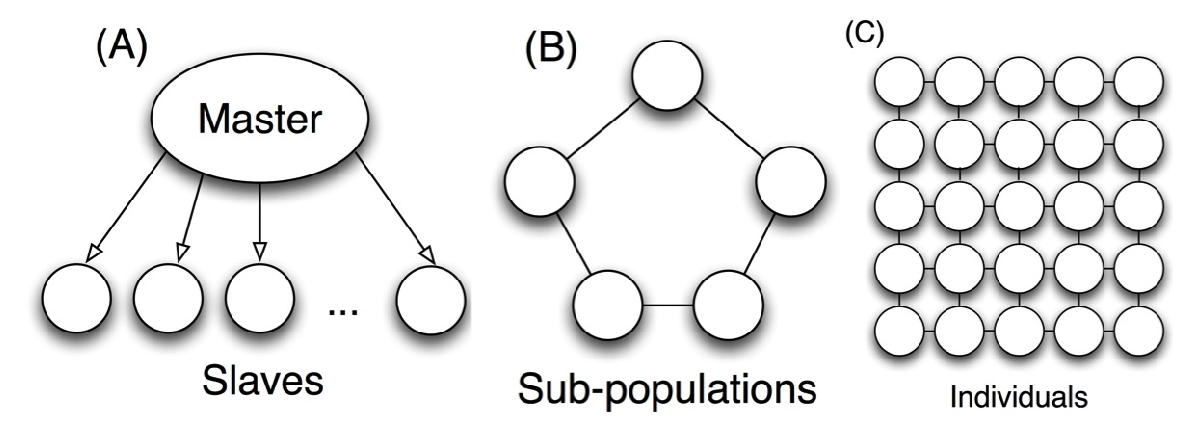
\includegraphics[width=0.7\textwidth]{Fig/Chapter2/PGA_reduced.eps}
        }
        \caption{Three different models of parallel genetic-algorithm: (A) master-slave, (B) coarse-grained, and (C) fine-grained.}
        \label{fig:PGA}
        \end{figure}

      Different from traditional genetic algorithm, the basic idea of parallel genetic algorithm is divide-and-conquer flavor, which can be applied to genetic algorithm in many different variations. Alba et al.~\cite{SurveyDistPGA1997} and Cant-Paz \cite{SurveyPGA1997} classify the parallel genetic algorithm into three main types: (1) master-slave genetic algorithm, (2) fine-grained genetic algorithm, and (3) coarse-grained genetic algorithm. Fig.~\ref{fig:PGA} shows three types parallel genetic-algorithm as mentioned above.
          
      Parallel genetic algorithm is not just parallel versions of traditional genetic algorithm, parallel genetic algorithm can actually reach the ideal goal via various parameters setting. Multi-objective optimization problem can achieved via different parameter and exchange their individuals between each sub-population.

    To elaborate the advantages of both deterministic optimization and circuit simulation, this work tends to integrated them as a hierarchical process. The framework inherit synthesis flow in \cite{PerfMap_ISQED2011} mostly. Here the updated flow replace the original performance exploration with PGA methodology. Also, the fine-tuning simulation is improve as probabilistic perturbation simulation. Therefore, our proposed flow is shown in Fig.~\ref{fig:PageFlow}, and the corresponding notations are list in the symbol list.

  \section{Device Fitting to Circuit-level Equation}
    At the beginning of synthesis framework, we have an abstraction from device model to circuit-level variables. Given the required devices of the target circuit design, the foundry device models provide such device characteristics with SPICE modeling. A set of analytical design equations are capable to map device-level variables into circuit-level design variables by modeling techniques such as symbolic analysis or curve fitting like~\cite{PWL_Convex_GP,Eeckelaert_DATE2003,Daems_DAC2002}. Two steps of technique accomplish the abstraction for design variables. 

    First of all, it is necessary to discover feasible variable values for each attendant device. In other words, all design variable values which cause device failed should be exclusive at this stage. By SPICE simulator, a matrix of accessible device level variable value are generated. However, since this step is collecting the feasible range of each device level parameters, the table is collected in one-time. 

    \begin{figure}[t]
      \centering
      \centerline{
        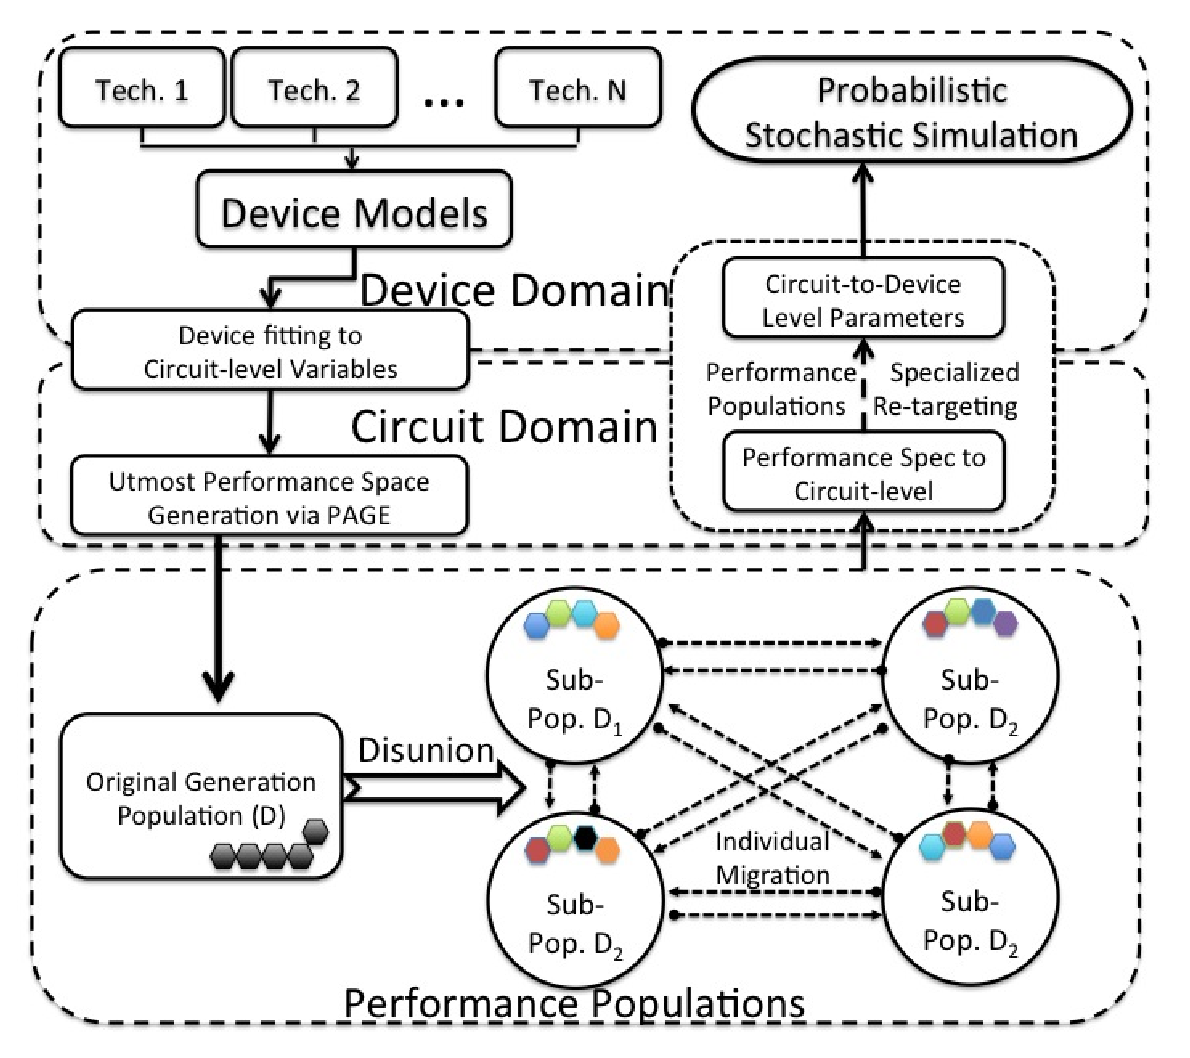
\includegraphics[width=0.7\textwidth]{Fig/Chapter2/PageFlow.eps}
      }
      \caption{Hierarchical performance exploration flow with PGA} 
      \label{fig:PageFlow}
    \end{figure}

    Secondly, such matrix of device-level variables are further mapped into circuit-level variables by curve fitting. An vivid example for design variable mapping is shown in Fig.~\ref{fig:DeviceFit}. Given a set of device-level variables $V^D= \{{v^D}_i| 1 \leq i \leq |V^D|\}$ , each $v^D_i$ has the same step number $S_{V^D}$ in each range. That is, while $v_i^D$ has maximum value $V^D_{MAX}$ and minimum value $V^D_{min}$, there should be $S_{V^D}$ values among then. Therefore, a set of feasible device-level variables are constructed in a matrix $T_{|V^D|\times S_{V^D}}$, where $T_{|V^D| \times S_{V^D}} = \{ t_{i,j}| 1 \leq i \leq |V^D|, 1 \leq j \leq S_{V^D} \}$. Meanwhile, a set of circuit-level variables $V^C = \{{v^C}_j| 1 \leq j \leq |V^C|\}$ should be extracted for performance exploration. As Eq.(\ref{eq:devToCir}),all training pairs of the extracted circuit-level variables from previous transformation and device-level variables are then formulated as least-square error problem in analytical posynomial form design equations to acquire fitting parameters.

    \begin{align}\label{eq:devToCir}
      \begin{array}[t]{rl}
        Variables: & \begin{array}[t]{rl}
                      T_{|V^D| \times S_{V^D}}  & = \{t_{i,j}| 1 \leq i \leq |V^D|,\; 1 \leq j \leq S_{V^D}\}   \\
                      V^C   &= \{v_j^C, 1\leq j \leq |V^C| \}   \\
                      v_j^C &= \{f_j^{(C_f)}(T_{|V^D| \times S_{V^D}})|1 \leq j \leq |V^C|\}  \\
                    \end{array} \\
         minimize & \| \sum{ v_j^C - f_j^{(C_f)}(T_{|V^D| \times S_{V^D}})}\|^2   \\
       subject\; to & C_f\in \left [{C_f}_{min}, {C_f}_{MAX} \right] 
      \end{array} 
    \end{align}

    where
    \begin{itemize}
      \item $C_f$ is the fitting parameters of $f_j$ 
      \item $\left [{C_f}_{min},{C_f}_{MAX}\right]$ is the range constraints of the fitting parameters in $f_j, 1 \leq j \leq |V^C|$.
    \end{itemize}

    Since parasitics are non-ignorable, the parasitic effects of devices should also be extracted for the following steps in order to exploit the trade-off between each aspect of circuit design variables and performance metrics.~\cite{Template_Based_Parasitic_Aware_Layout}. The problem formulation is similar to Eq.(\ref{eq:devToCir}) in Eq.(\ref{eq:paraExt}):
    \begin{align}\label{eq:paraExt}
      \begin{array}[t]{rl}
      Variables:  & \begin{array}[t]{ll}
                      T_{|V^D| \times S_{V^D}} &= \{t_{i,j}| 1 \leq i \leq |V^D|,\; 1 \leq j \leq S_{V^D}\}   \\
                      V^P     & = \{v^p_l|1 \leq l \leq |V^P|\} \\
                      v^p_l   & = \{Q_l^{(C_p)}(T_{|V^D| \times S_{V^D}})| 1 \leq l \leq |V^P| \}
                    \end{array} \\
      minimize    &  \| \sum{v^p_l-Q_l^{(C_v^p)}(T_{|V^D| \times S_{V^D}})}\|^2  \\
      subject to  &  C_v^p \in \left [ {C_v^p}_{min}, {C_v^p}_{MAX}\right] 
      \end{array} 
    \end{align}

    where
    \begin{itemize}\setlength{\itemsep}{2pt}
      \item $v^p_l$ is the mapping equations from $T_{|V^D|\times S_{V^D}}$ to $V^P$, 
      \item $C_p$ is the fitting parameters of $Q_l$,
      \item $\left [ {C_{v^p}}_{min}, {C_{v^p}}_{MAX}\right]$ is the range constraints of the fitting parameters in $Q_l$.
    \end{itemize}

    \begin{figure}[t]
      \centering
      \centerline{
        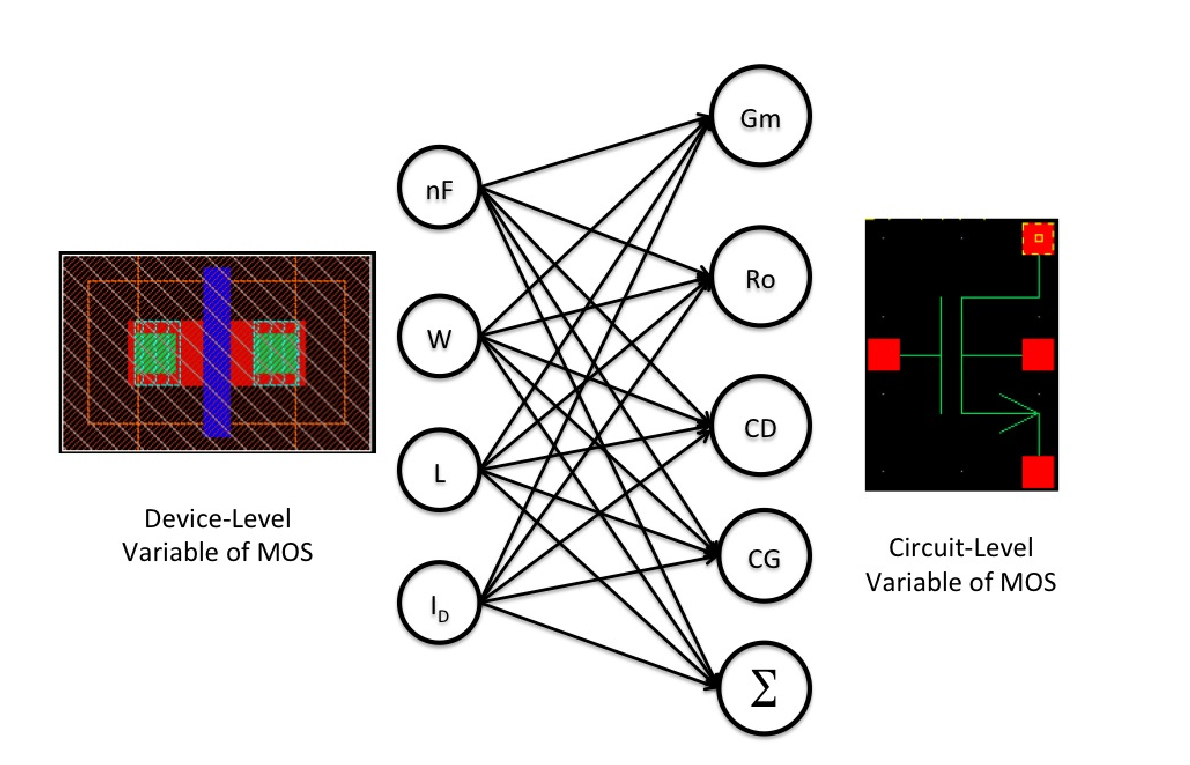
\includegraphics[width=0.7\textwidth]{Fig/DeviceFit.eps}
      }
      \caption{Mapping device-level variables of one NMOS(number of fingers, device channel width/length and current) to circuit-level variables ($G_m$, $R_o$, $C_D$, $C_G$ and $\Sigma$) } 
      \label{fig:DeviceFit}
    \end{figure}

  %!TEX root = Thesis.tex

  \section{Performance Space Exploration with Parallel Genetic Algorithm}\label{sec:pga}
    
    \begin{figure}[t]
      \centering
      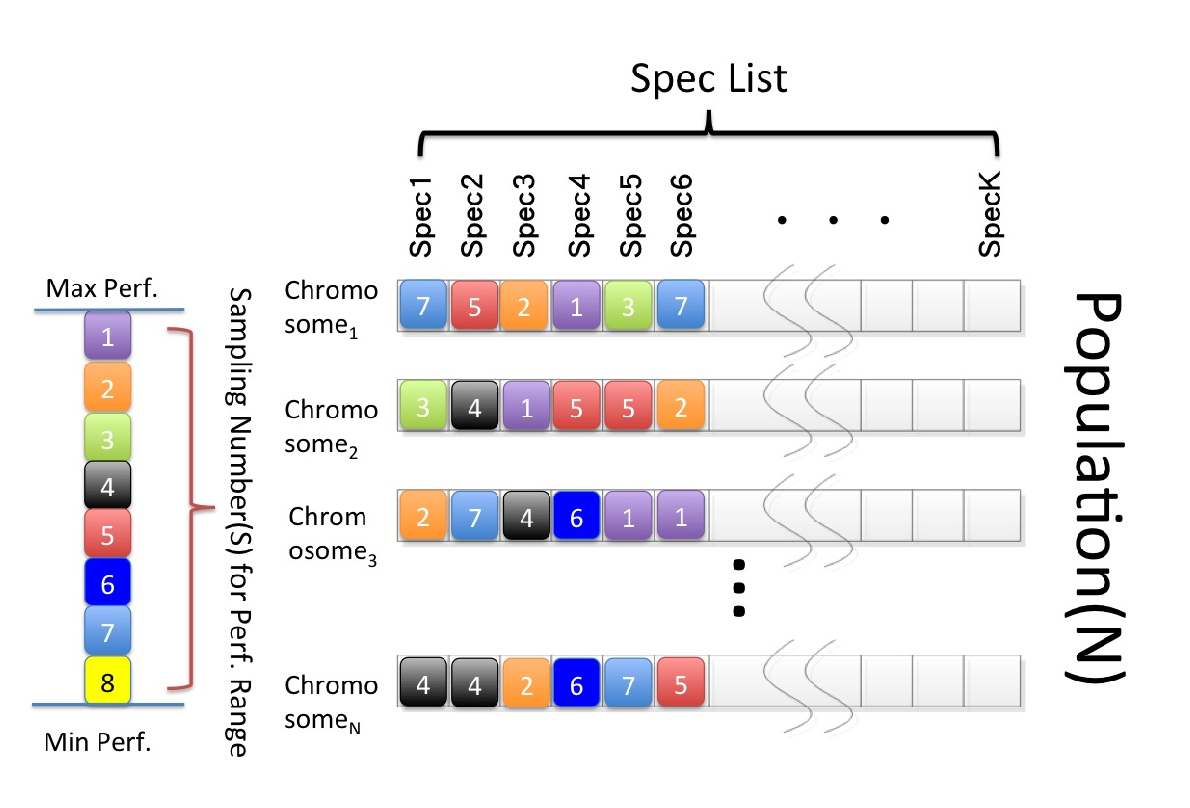
\includegraphics[width=\textwidth]{Fig/Gene.eps}
      \caption{Demonstration of genetic representation for performance metrics.} 
      \label{fig:Gene}
    \end{figure}

    To traverse the space of required circuit performance, we propose an efficient exploration process to investigate the feasible performance metrics of such analog design. Once the set of circuit-level design variables $V^C$ are prepared, these variables can be adopted as parameters into circuit design equations. A set of design equations along with circuit-level parameters, parasitic effects and fitting parameters are constrained with performance requirement. Note that the parasitic effects of the devices are included so as to explore the trade-off between each aspect of performance metrics and circuit-level design variables. To figure out the design equation set with performance constraints is feasible or not, we apply convex optimization. Since the circuit design equations are formulated as geometric programming by posynomial forms, the optimization to find feasible solution with performance constraints is convex. Moreover, to extend the problem with different performance specifications, that each combination of performance constraints can be checked is feasible or not. A set of specification are swept as the constraints for an optimization performance to get performance metrics.
 
    An optimization problem in Eq.(\ref{eq:DesignEq}) describes a unit performance optimization step.

    \begin{align}\label{eq:DesignEq}
      \begin{array}{ll}
      Variables:  & \begin{array}[t]{ll}
                        V^C & = \{{v_k}^C | 1 \leq k \leq |V^C|\} \\
                        V^P   & = \{ v^p_k | 1 \leq k \leq |V^P| \}\\
                        F   & = \{ f_k | 1 \leq k \leq |F| \}\\
                        R   & = \{ r_k | 1 \leq k \leq |R| \} 
                    \end{array}                 \\
        minimize  &   f_{OBJ}( {v_i}^C,v^p_k,f_k)         \\
      subject\ to & \begin{array}[t]{l}
                    r_1 = Perf_1(V^C,V^P,F) \geq z_1\\
                    r_2 = Perf_2(V^C,V^P,F) \geq z_2\\
                    \vdots \\
                    r_k = Perf_k(V^C,P,F) \geq z_k
                \end{array}             
      \end{array}
    \end{align}
    where
    \begin{itemize}
      \item  $V^C$ is circuit level variables extracted from device-level variables.
      \item  $V^P$ is a set of parasitics which is non-ignorable for circuit modeling.
      \item  F demonstrates fitting parameters to fit from circuit-level parameters to performance space.
      \item  R represents the corresponding performance result set which obtain by optimization. 
      \item  $Z = \{z_k| 1 \leq k \leq |Z|\}$ is a set of performance required value. In other words, each $z_k$ represents a value of performance constraint, eg. $z_k \geq 40 \to Av \geq  40dB$
    \end{itemize}
    \vspace{0.3cm}

  
    In every optimization process, one performance metric results in a set of performance metric ($r_1 ,\ldots, r_k$) corresponding to the given specification of performance($z_1,\ldots,z_k$). Therefore, according to the same design equation for optimization, it is an one to one mapping relationship from spec to result of performance and the corresponding circuit-level design variables. 

    To extend the optimization range. Each $z_k$ can be varied with a range of value, that is, we define a maximum value of $z_{kMAX}$ and one minimum value of $z_{kmin}$ with several step value between them. Therefore, we can investigate the performance limitation for $z_k$ by implementing optimization on a series of $z_k$, $z_k=\{z_{ki}| 1 \leq i \leq |z_k|, z_{kMAX} \leq z_{ki} \leq z_{kmin} \}$. Obviously, a set of different performance types with a range of such values are similar to chromosome concept in heredity. As we can see in Fig.~\ref{fig:Gene}, if every chromosome carries different value of every performance metric $z_k$. An evolutionary computing with genetic algorithm for traversing solution space can be employed for traversing optimized multi-objective problem. As mentioned in Section~\ref{sec:PGAIntro}, we further utilize the {\it Parallel Genetic Algorithm} to develop with. The detail implementation is as follows:

    


    \subsection{PGA Overview}

      The methodology to exercise PGA fusion with performance exploration is shown in Algorithm~\ref{alg:PGA}. PGA traverses the performance space by evolution. According to \cite{SurveyDistPGA1997}, our approach picks the coarse-grained fashion PGA. In traditional genetic algorithm, one major population has numbers of individual chromosomes for evolution. In coarse-grained genetic algorithm, the major population is separated into numbers of sub-populations with the same size of individual. Since each sub-population contains large number of individuals, it is time-consuming to exercise fine-grained structure. Therefore, the coarse-grained structure is much efficient at this situation. 


      \begin{figure}[t]
        \centering
        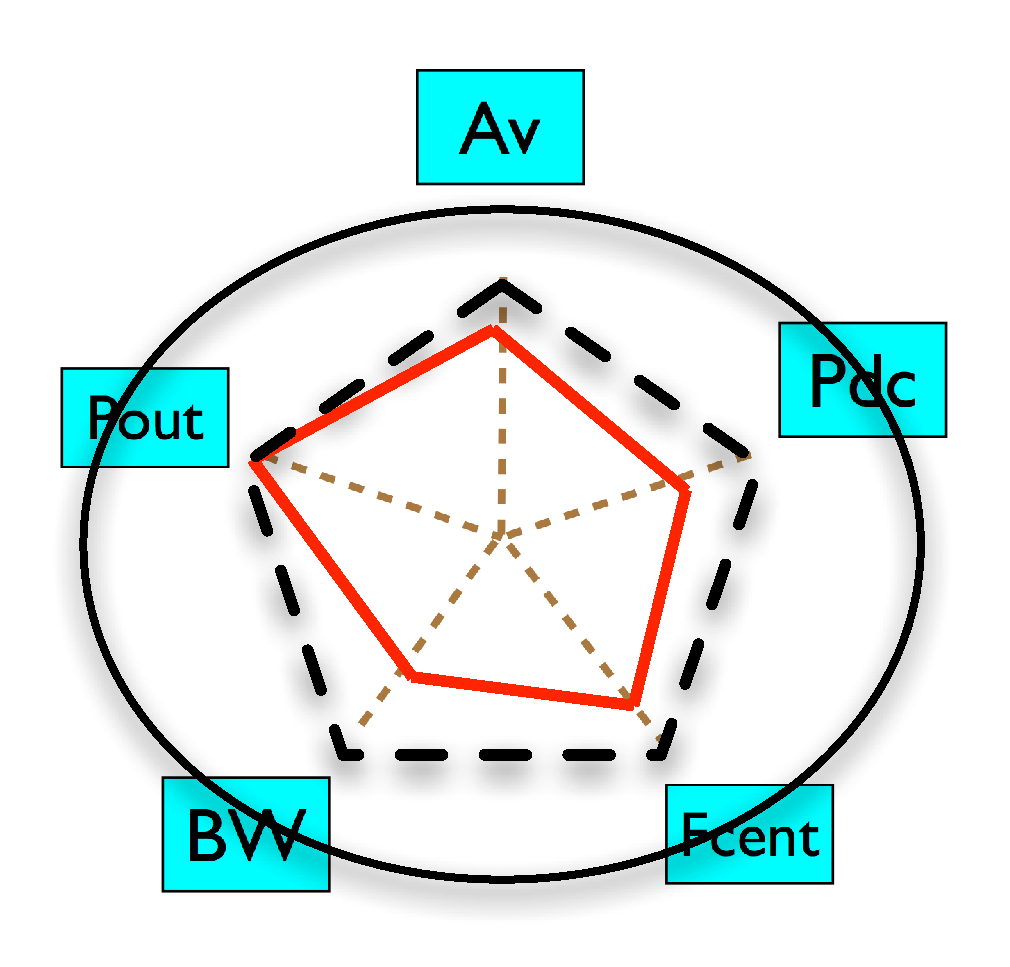
\includegraphics[width=\textwidth]{Fig/MultiSpec.eps}
        \caption{Illustration of performance characteristic (e.g., Av, Pdc, Pout, BW, Fcent, etc.) for each circuit.} 
        \label{fig:MultiSpec}
      \end{figure}


      \newcommand{\PGA}{\ensuremath{\mbox{\sc PGA}}}
      \algloopdefx{RETURN}[1][]{\textbf{return} #1}
      \algblockdefx{FORALLP}{ENDFAP}[1]%
      {\textbf{for all }#1 \textbf{do in parallel}}%
      {\textbf{end for}}
      \begin{algorithm}[t]  
        \caption{$\PGA(Z_{K\times S},N_P,S,k,T,C,M_P)$}\label{alg:PGA}                       
        \begin{scriptsize}
          \begin{algorithmic}[1]
            \REQUIRE 
              \begin{tabular}{l}
              $Z_{K\times S}$: Performance Space Matrix. \\
              $N_P$: Number of Individuals in major population.\\
              %$N_S$: Number of sub-populations.\\
              S: Sampling number for each performance spec $z_k$\\
              K: Number of Performance spec type\\ 
              T: Technology type. \\
              C: Circuit type.\\
              $M_P$: Migration rate.
                \end{tabular}
            \ENSURE 
              \begin{tabular}{l}
                $R_{K \times S}$ : The result performance space\\
                    $P$ : The population of performance specs after PGA
                  \end{tabular}
              \FOR {$i = 1 \to N_P$}
                \FOR {$j = 1 \to k$}
                  \STATE $G_i \gets RandGetSpec(Z_{j\times S})$ \COMMENT{Randomly generate spec value from Z}   
                \ENDFOR
                \STATE $P \gets G_i$
              \ENDFOR
              \FOR {$i = 1 \to k$}
                \STATE $P_i \gets Partition(P,i)$
              \ENDFOR
              \WHILE {Convergence criterion satisfied}          
                \FORALLP {$i = 1 \to k$} 
                  \STATE $R_i \gets Evaluate(P_i,T,C)$
                  \STATE ${Pool}_i \gets Reproduction(P_i,Fitness(T,C,i,R_i))$
                  \STATE $P_i \gets Crossover(P_i,{Pool}_i)$
                  \STATE $P_i \gets Mutation(P_i)$
                \ENDFAP   
                \FOR {$i = 1 \to k$} 
                  \STATE $Migration(P_i,exclusive(P,P_i),M_P)$
                \ENDFOR 
              \ENDWHILE
              \STATE $P \gets Merge(P_1,P_2, \ldots, P_{k})$
              \RETURN $P, R_{K \times S}$  
          \end{algorithmic}
          \end{scriptsize} 
      \end{algorithm}

      As for analog performance optimization, which is a multi-objective problem with a Pareto-front as illustrated in Fig.~\ref{fig:MultiSpec}. To find the Pareto-front, each performance target optima should be traverse as well. Therefore, we further use heterogeneous coarse-grained structure for evolution. In other words, every sub-population deals with different objective that performs optima. For example, one sub-population implement performance exploration to evolve population with better voltage gain($A_v$). Therefore, we pick the fitness function which emphasizes on such performance item($A_V$). Moreover, each sub-population has its own fitness function and evolve independently. Additionally, the diversity for the overall population also can be maintain by migration strategy in the end of the performance exploration stage.

    \subsection{Chromosome Encoding}

      Before PGA process, the fundamental chromosome encoding should be defined. For one performance target $z_k$, given performance upper and lower bound, $\{\left [z_{kmin},z_{kMAX} \right]$. There exist a set of discrete $z_{k,s}$ among this boundary, where 
      \begin{defi}\label{def:Z}
        $\forall z_k, \exists z_{k,s} \to z_{k,S} = \{z_{kmin} \leq z_{k,s} \leq z_{kMAX}\}$. As Algorithm~\ref{alg:PGA} mentioned in $Input:$, S denotes the sampling number for each $z_k$. Therefore, $z_{k,s} = \{z_{kmin} + ({z_{kMAX}-z_{kmin}})\times s/S | 1 \leq s \leq S\}$
      \end{defi}

      \begin{align}\label{eq:PerfMatrix}
        \begin{array}{rl}
          Z_{K \times S} & = 
              \left[\begin{array}{cccc}
               z_{11} & z_{12} & \dots  & z_{1S} \\
               z_{21} & z_{22} & \dots  & z_{2S} \\
               \vdots & \vdots & \vdots & \vdots  \\
               z_{K1} & \dots  & \dots  & z_{KS} 
            \end{array}\right]
        \end{array}
      \end{align}
   
      where
      \begin{itemize}
        \item K: the number of performance specification types. (eg: Av, BW,...,etc.)
        \item $\left[Z_{min},Z_{MAX}\right]_{k}$, $k = 1, \ldots, K$ is the $k_{th}$ type specification range of the performance space.
        \item S is the sampling number for each $Z_S$ between ${Z_k}_{min}$ and ${Z_k}_{MAX}$.
        \item  $\forall z_{ki} \in Z_{K \times S}$, if $i= 1$, $z_{ki}= {Z_S}_{min}$ and if $i = S$, $ z_{ki}={Z_S}_{MAX}$
      \end{itemize}

      By Definition~\ref{def:Z}, every $z_{k,s}$ for $z_k$ are selected as constraints for an optimization problem which represents the circuit design equation. Here we expand the performance space as an $S \times N$ matrix in Eq.(\ref{eq:PerfMatrix}). Moreover, each performance spec from constraints is is encoded as chromosome G from maximal to minimal in a set of $G = \{g_k| 1 \leq k \leq K\}$. For example, $g_i \in G$ randomly obtains value of the $k^{th}$ spec from $z_{k,1}$ to $z_{k,S}$.

    \subsection{Initialization}
      As algorithm~\ref{alg:PGA} described in $Input$, a set of performance space matrix $Z_{K \times S}$ is given. First of all, a major population is constructed according to $Z_{K \times S}$. Algorithm~\ref{alg:PGA} Line 1 to Line 6 illustrate the process to assign performance specs as chromosome for each individual of the major population iteratively. For the reason that we want to achieve multi-objective optimization, k sub-populations are generated and evolved independently. Therefore, a major population $P$ is generated. According to the size of sub-population $k$, master processor allocates individuals to each slave processor uniformly as sub-population $P_1 \ldots P_{k}$. 
  
    \subsection{Evolution}

      An evolution is executed between Algorithm~\ref{alg:PGA} Line 10 and Line 20. Because the $Evaluate$, $Reproduction$, $Crossover$ and $Mutation$ parts are independent, the parallel parts can be performed from algorithm~\ref{alg:PGA} Line 11 to Line 16. Hence, in each sub-population, each location of gene in one individual is fed into $Evaluate(P,T,C)$ as target constraints for performance to the design equation(shown in Eq.(\ref{eq:DesignEq})) and a corresponding result $R_i$ is obtained. However, if one combination of performance metrics produces the solution space which is not convex, such individual would be failed by $Evaluate$. Then, a random generated individual replaces and redoes $Evaluate$ again until each chromosome $G$ has obtained its corresponding result $R = \{r_k| 1 \leq k \leq|R| \}$. 
      
      Fig.~\ref{fig:PGAFlow} shows the flow of the parallel genetic evolution from random performance space matrix($Z_{K\times S}$) to convergence. Each sub-population experiences a evolution with $Evaluate$, $Reproduction$, $Crossover$ and $Mutation$. Between algorithm~\ref{alg:PGA} Line 12 to Line 15, parallel genetic algorithm utilizes a fitness function to determine the suitability for each $G_i$. In our algorithm, we use the $Heterogeneous\ Island$ architecture \cite{SurveyCGPGA1994}. According to our requirement, we tend to specialize the particular spec, such as voltage gain($A_v$). A set for fitness function is given, $Fitness = \{{fitness}_i| 1 \leq i \leq k\}$ as kind of objective function to determine how important each individual is with the $Evaluate$ result. Each sub-population $P_i$ applies one particular fitness function which is related to the required performance result $R_k$ of $Evaluate$ value. Therefore, the fitness function determines the qualified individuals to be preserved to the crossover pool in a weighted ratio, and the others should be extinct. In $Crossover$ of algorithm~\ref{alg:PGA} Line 14, the $Crossover$ step selects each two genes $G_i$ and $G_j$ ,where $\{G_i,G_j \in Pool; 1 < i<j<N\} $ for copulation. Since each individual has $K$ types of spec, these two individuals exchange {\bf c} specs and reserve {\bf $K-c$} specs with each other. In the end of parallel sub-level evolution, the {\it Mutation} step picks up one individual with mutation rate and then replaces one gene value by one slot of $Z_K$. 
    
      \begin{figure}[t]
        \centering
        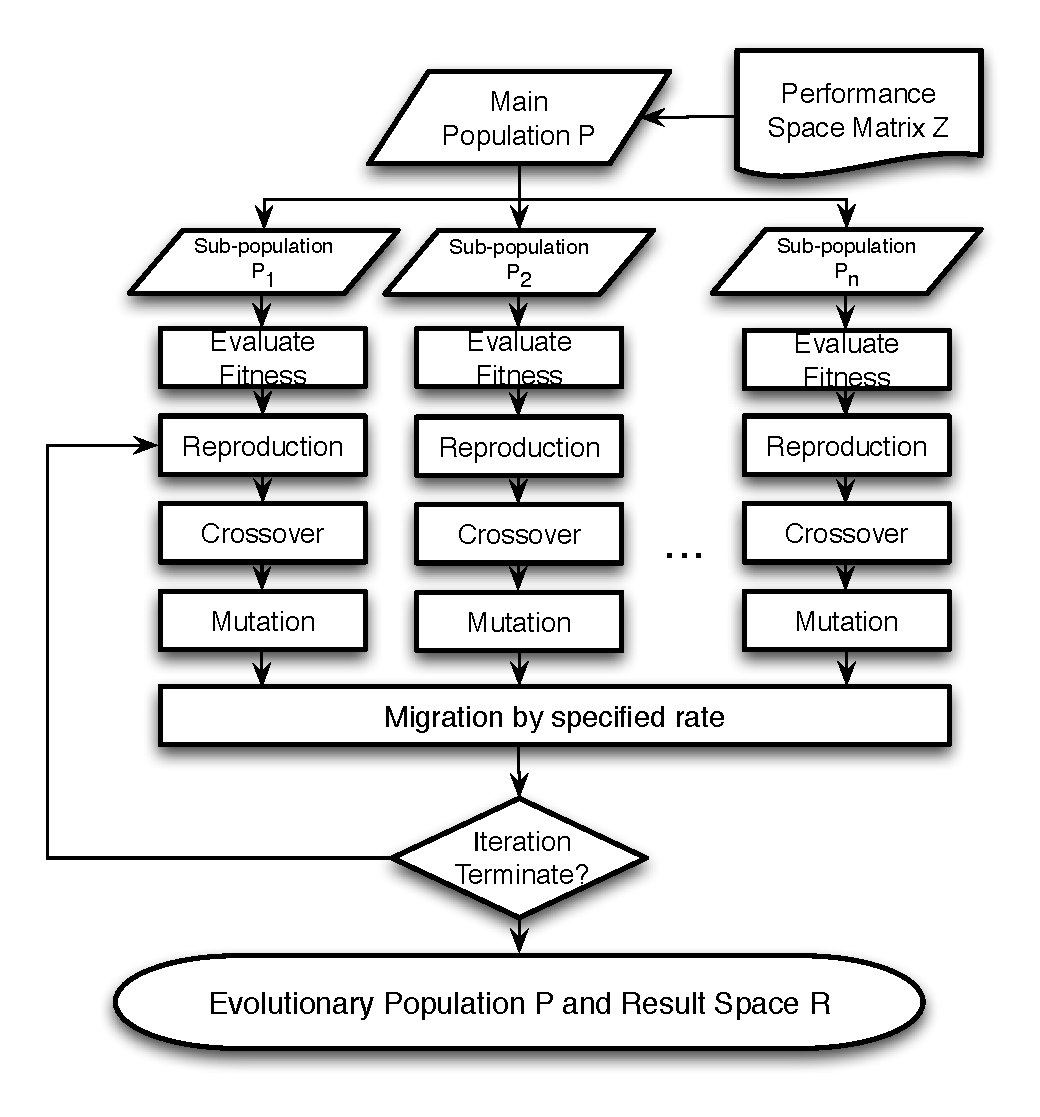
\includegraphics[width=\textwidth]{Fig/PAGEflowchart.eps}
        \caption{Coarse-grained parallel genetic approach from major population P to partitioned population $P_i$ for parallel evolution. The migration step benefits each sub-population on diversity every iteration.} 
        \label{fig:PGAFlow}
      \end{figure}

    \subsection{Migration}  

      \newcommand{\Migration}{\ensuremath{\mbox{\sc Migration}}}
      \algloopdefx{RETURN}[1][]{\textbf{return} #1}
      \algblockdefx{FORALLP}{ENDFAP}[1]%
      {\textbf{for all }#1 \textbf{do in parallel}}%
      {\textbf{end for}}
      \begin{algorithm}[t]  
        \caption{$\Migration(P_i,exclusive(P,Pi),M_P)$}\label{alg:Migration}                       
        \begin{scriptsize}
          \begin{algorithmic}[1]
            \REQUIRE 
              \begin{tabular}{l}
              $P_i$: The population which want to migration, where $i = 1... k$\\
              $exclusive(P,P_i)$: Return a population set except $P_i$ .\\
              %$N_S$: Number of sub-populations.\\
              $M_P$: Migration rate.
                \end{tabular}
            
              \FOR {$j = 1 \to k$}
                  \IF{$j \neq i$}
                    \STATE $R_P \gets rand(0,1)$
            \IF{$R_P \leq M_P$}
                      \STATE  $I_S=bestIndividual(P_i,fitness(T,C,j,R_i))$
              \STATE  $I_R=worstIndividual(P_j,fitness(T,C,j,R_j))$
              \STATE  $replaceIndividual(P_i,P_j,I_S,I_R)$
            \ENDIF
          \ENDIF
                \ENDFOR
             
              \STATE $P \gets Merge(P_1,P_2, \ldots, P_{k})$
              
          \end{algorithmic}
          \end{scriptsize} 
      \end{algorithm}

      In the end of each independent evolution, we perform $Mutation$ with a given mutation rate for sub-population $P_i$ from 1 to $K$. Later, every sub-population is updated. Then, $Migration$ is summarized as shown in Algorithm~\ref{alg:Migration} aims to exchange individuals in the population network shown in the bottom of Fig.~\ref{fig:PGAFlow}. Therefore, each $P_i$ should operate $Migration$ with the others. From algorithm~\ref{alg:Migration} Line 5 to Line 7, each $Migration$ between $P_i$ and $P_j$, $P_i$ exchanges its best individual with respect to ${fitness}_j$, and $P_j$ replaces its worst individual with respect to own ${fitness}_j$ with migration rate $M_P$ in algorithm~\ref{alg:Migration} Line 4. Different sub-population owns its fitness function and uses the particular migration strategy can close to natural evolution. An example of a migration operation between two sub-populations is shown in Fig.~\ref{fig:Migration}. After the $Migration$ is executed, the composition of each $P_i$ is updated with higher diversity. 
    
    \subsubsection{Merge}
      After all, while the termination condition meets, all the sub-populations are generated. These sub-populations not only have good solution with respect to all spec, but also enhance diversity. All individuals in each sub-population merge to a main population one after another. After merge, main population has all the individuals generated from evolution. 
  
  
      \begin{figure}[t]
        \centering
        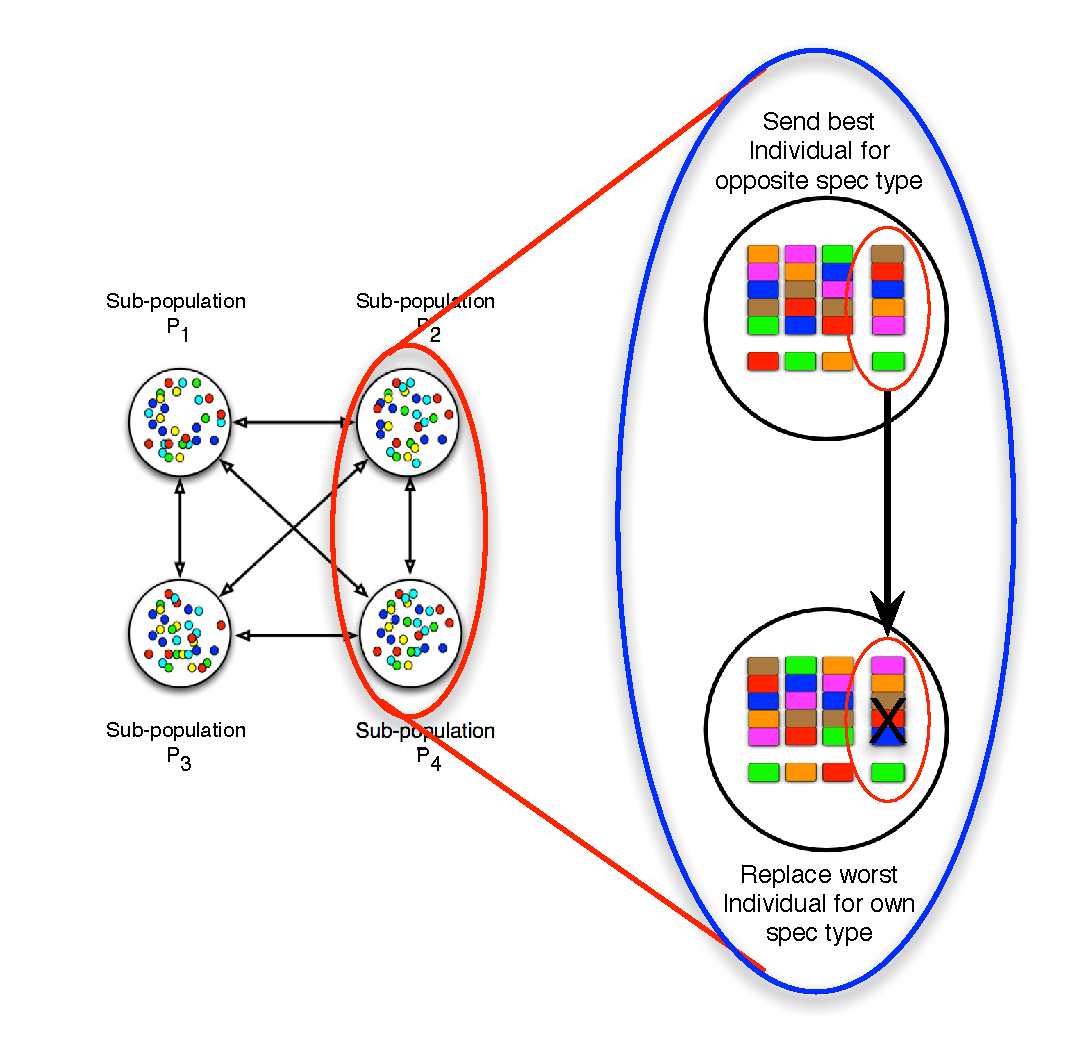
\includegraphics[width=\textwidth]{Fig/PAGEMigration.eps}
        \caption{When sub-population $P_2$ and sub-population $P_4$ perform migration operation with migration rate $M_P$, $P_2$ sends its best individual with respect to spec type $P_4$, and the receiving sub-population $P_4$ replaces its worst individual with respect to its own spec type $P_4$.} 
        \label{fig:Migration}
      \end{figure}

    To consider the complexity of PGA, it is considerable to check the dimension of $Z_{K\times S}$. According to line 12 in Algorithm~\ref{alg:PGA}, $Evaluate(P_i,T,C)$ is the most critical. Each $Evaluate$ for $P_i$ need to resolve $\frac{N_P}{N_S}$ convex optimization problems in serial, which is $O(\frac{N_P}{N_S})$. Comparing to the exhaustive approach, the complexity is restricted to $K$ and $S$. That is, we need to traverse every combination from specification space in $Z_{K\times S}$ for $O(S^K)$ complexity. For example, if a circuit require two performance specs ($A_v$ and $BW$) with 4 sampling steps ($A_v = \{5,10,15,20\}$, $BW = \{3MHz,5MHz,8MHz,10MHz\}$). Therefore, the overall combination of specs need to be checked is $4^2=16$. Obviously, we can observe the gap with more specs($K\uparrow$) and greater precision in sampling($S\uparrow$). To sum up, a genetic-based approach can reduce the complexity by controlling population number and a parallel enhancement further reduce the timing complexity vi parallel number. However, the accuracy is also sacrificed as trade-off.



\label{sec:GPEF}

  \section{Performance Space Re-targeting to Design Variables}\label{sec:reTarg}
    
    After generating specialized populations by PGA evolution, it comes to a reverse interpolation from a series of performance specifications through circuit-level design variables to device-level design variables. Hence, K groups of optimal-potential performance spaces of the circuit under chosen technology are traversed. Since a set of performance metrics directly represents the limitation of specifications, such group of optimal performance specification is locked from optimal performance. Ideally, the optimization engine should be capable of directly finding the geometry-biasing-level design variables. 

    Next, we want to find the optimal candidates of device-level design variables. From previous stage, the circuit-level design variables are obtained. Here the distribution of the device-level design variables are also obtained through this design re-targeting stage. As Eq.(\ref{eq:SingleReTarg}) illustrated, since each device has its particular device variables, all of them are considered for optimization. $M$ stands for a set of attendant devices in the circuit. Generally, each device has different number of variables. Therefore, $V^D_{m_k}$ represents the variable set of single $m_j$. Referring to Section~\ref{sec:pga}, Performance results $R_{S \times K}$ are obtained along with the same number($N_P$) of $V^C$ and $V^P$. Each $v^C$ and $v^P$ will re-target to a set of device-level parameter values via $f_{RE}(v^C, v^P)$ transformation. Eq.(\ref{eq:SingleReTarg}) shows a single transformation from each $v^C$ and $v^P$ to a set of device-level parameters $V^D_M$,

    \begin{align}{\label{eq:SingleReTarg}}
      \begin{array}[t]{rl}
        Variables & \begin{array}[t]{rl}
                      M         &= \{ m_j| 1 \leq j \leq |M|\} \\
                      V^D_M     &= \{ v^D_{m_j} | 1 \leq j \leq |M|\} \\
                      v^D_{m_j} &= \{v^D_{m_{j,k}}| 1 \leq k \leq |v^D_{m_j}|\}\\
                      v^C       &= f^{(C_f)}(V^D_M)\\
                      v^P       &= Q^{(C_Q)}(V^D_M)\\
                    \end{array} \\
         minimize & Q(V^D_M \to V^P)  \\
       subject\; to & V^D_M\in \left [{V^D_M}_{min}, {V^D_M}_{MAX} \right] 
      \end{array} 
    \end{align}

    \begin{figure}[t]
      \centering
      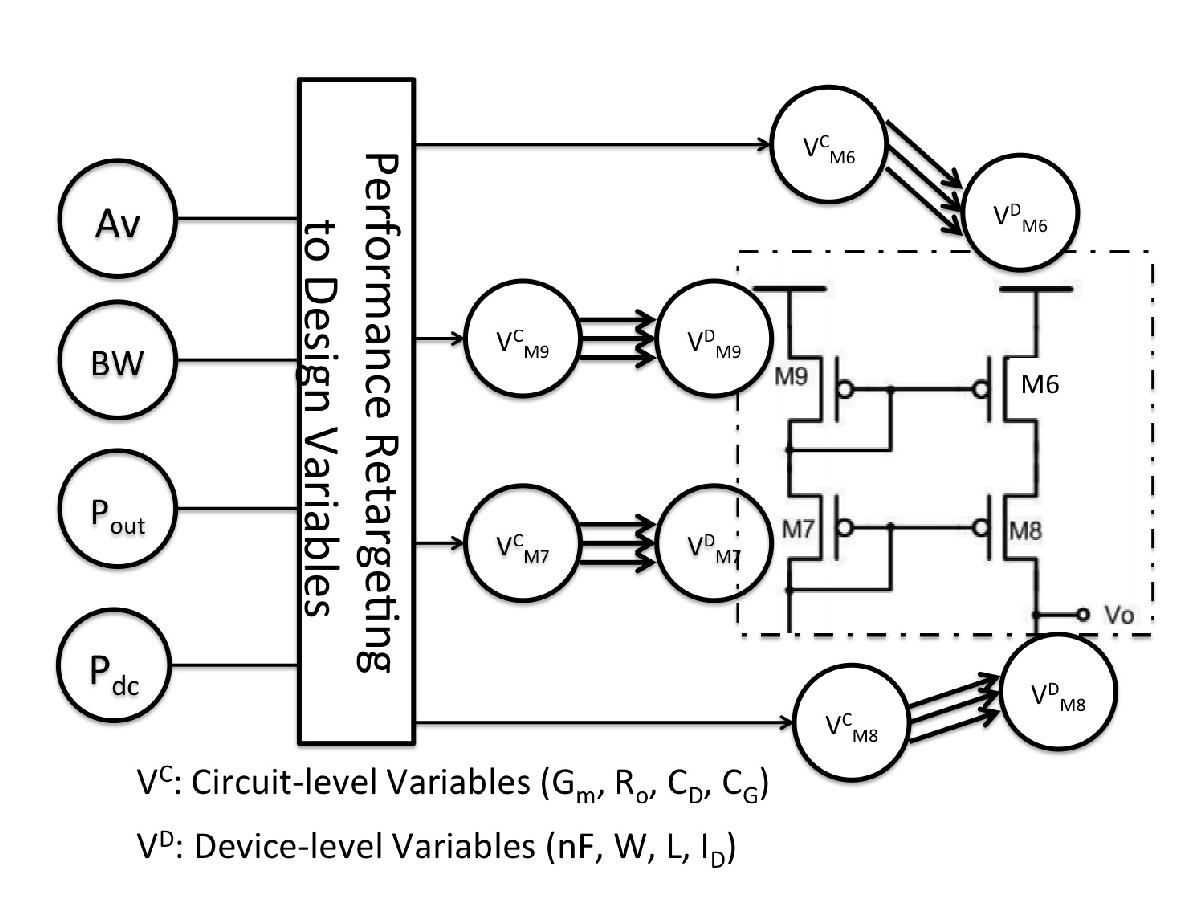
\includegraphics[width=0.7\textwidth]{Fig/Chapter2/Retarg.eps}
      \caption{Given merged populations of performance specs, a reversed process is to retrieve the corresponding design variables of each device (PMOS) in the circuit for optimal sizing values.} 
      \label{fig:Retarg}
    \end{figure}
    
    In Eq.(\ref{eq:SingleReTarg}), $Q$ is a cost function that involves the parasitic effects of the device, such as a product of area, parasitic cap/resistance, or self-resonance frequency, etc. For all, Every individual $V^C$ and $V^P$ need to be transfer to device-level parameters as distributions. In Eq.(\ref{eq:FullReTarg}), $\Psi$ collects $N_P$ set of device variables for required circuit.

    \begin{align}{\label{eq:FullReTarg}}
      \begin{array}{l}
        V^C = \{v^C_i| 1 \leq i \leq N_P\}\\
        V^P = \{v^P_i| 1 \leq i \leq N_P\}\\
        \Psi =  \{V^D_{M_{i,j,k}}| 1\leq i \leq N_P, 1 \leq k \leq |M|, 1 \leq j \leq |v^D_{m_k}|\} 
      \end{array}
    \end{align}

    Also, as shown in Fig.~\ref{fig:Retarg}, multiple solutions as distributions are generated from {\it Performance Space Exploration} in Section~\ref{sec:pga}, and it stands for a set of potential parameters for devices in required circuit. However, $\Psi$ not only narrows down the solution space for circuit simulation, but provides good prediction for optimal performance which will be validated via probabilistic simulation in Section~\ref{sec:ProbSimu} efficiently. 

  %!TEX root = Thesis.tex
                                            
\section{Effective Probabilistic Fine Tuning}\label{sec:pss}


  The final refinement performs a full-circuit stochastic simulation. Although we obtain a set of potential design variables from Section~\ref{sec:reTarg}, these do not represent the optimal solution. The final refinement performs simulation to prevent the solution from any non-ideal effects via higher-level abstraction. After {\it Design Re-targeting}, a set of overall device level variable values $\Psi $ are collected. $N_{V^D}$ collects the number of all device variables type. Since these design variables are selected by performance exploration via transformation, each population of performance metrics directly projects to a set of variable distribution. Basically, $\Psi$ provides the variable space for perturbation. By swapping among device-level parameters, the cost of full-circuit simulation is reduced. By employing global optimization algorithm, such as random walk or simulated annealing, the entire circuit is re-constructed and fed into circuit simulator using real models and parameters from the foundry.

  \begin{figure}[t]
      \centering
      \begin{subfigure}[t]{0.4\textwidth}
        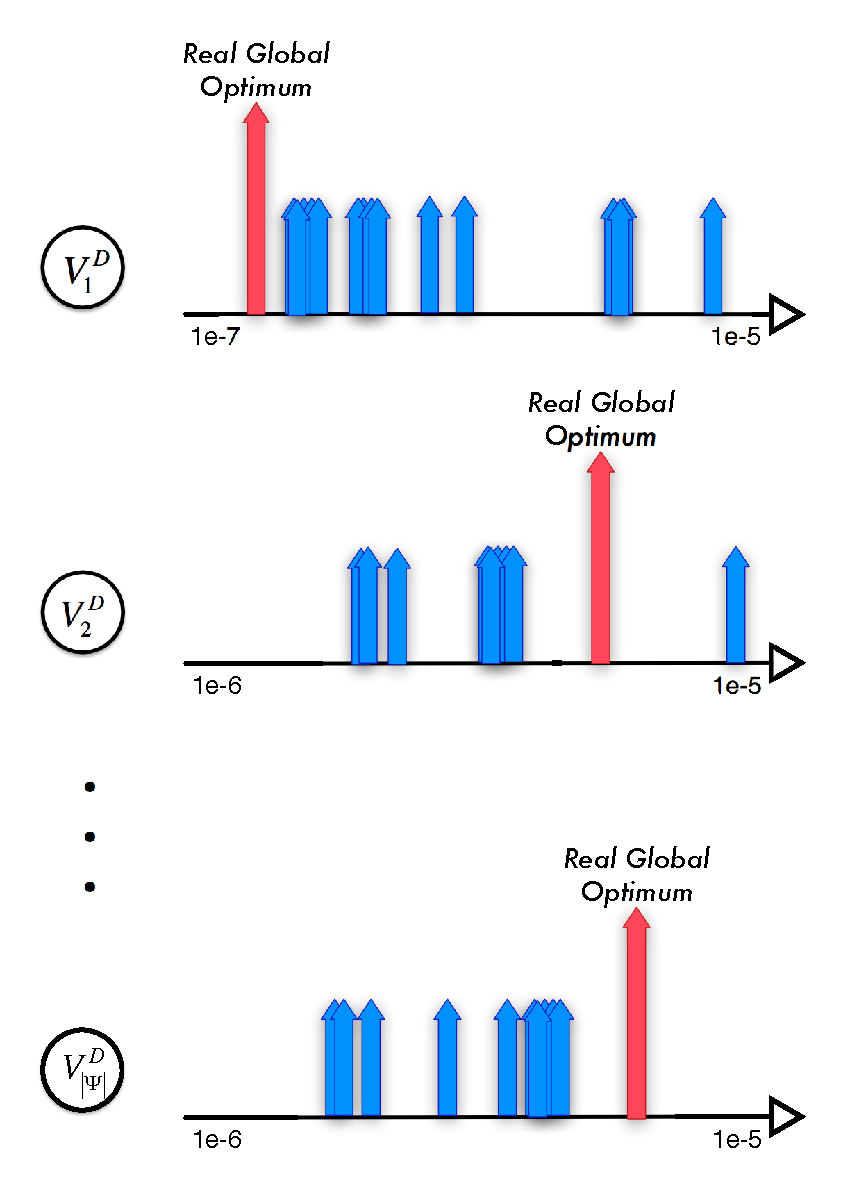
\includegraphics[width=\textwidth]{Fig/popSampling.eps}
      \end{subfigure}
      \begin{subfigure}[t]{0.4\textwidth}
        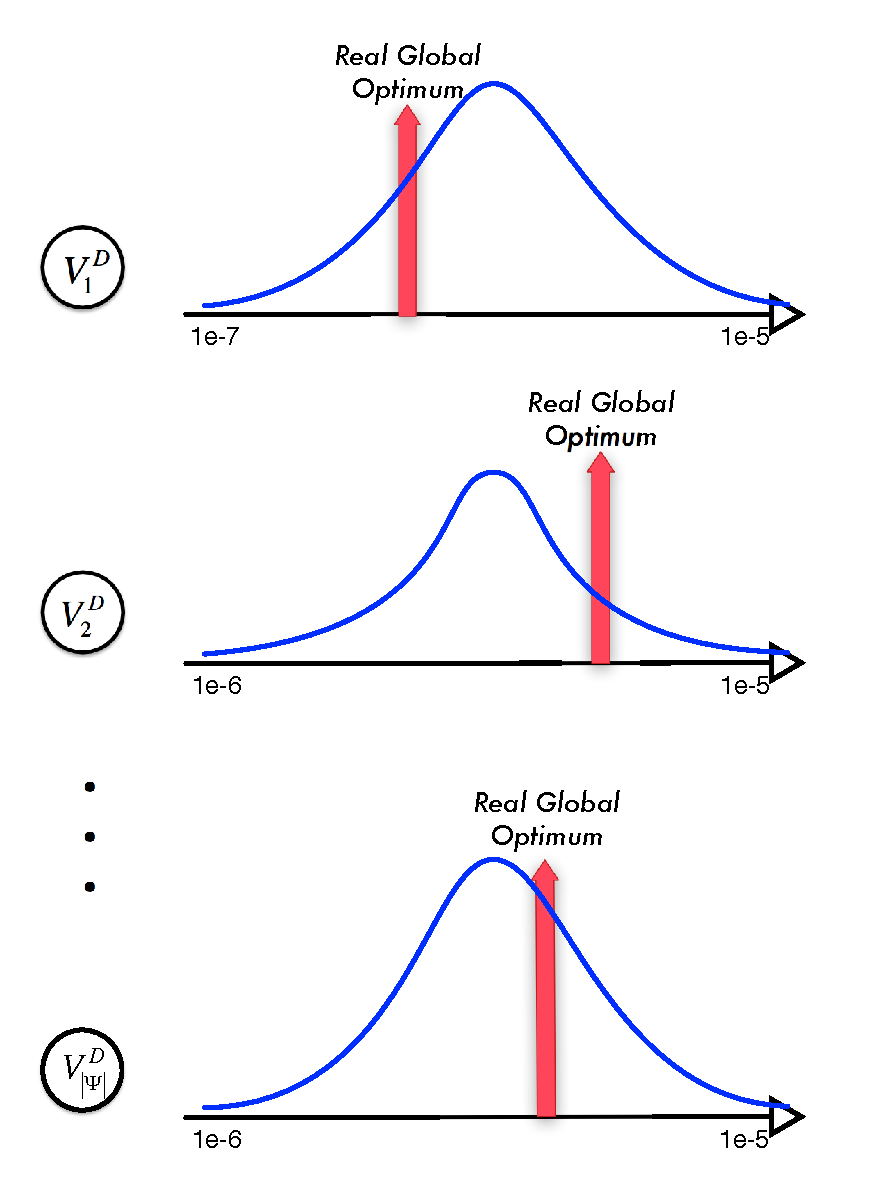
\includegraphics[width=\textwidth]{Fig/norPopDis.eps}
      \end{subfigure}
      \caption
      {
        Different distribution for stochastic simulation. (a) Population samplings for each device level variable from population and the global optimum location. (b) Normal distributions for each device level variable after normalized and the global optimum location.
      }\label{fig:optimumValleys}
  \end{figure}

  Such multi-objective simulated annealing (SA) based stochastic simulation is implemented in \cite{PerfMap_ISQED2011}. During perturbation, each swap of $V^D_m$ is referred to a uniform manufacturable range with respect to each device variable ($V^D_{M_{min}},V^D_{M_{MAX}}$). Since the range of each device variable is uncertain and continuous, the solution set can be wide. Normally, a movement among the range of $V^D_M$ is decided by the uniform probability, i.e., every movement is randomly chosen in the equal chance. As a matter of fact, some corner values are trivially unfeasible, and it is time-consuming to evaluate unfeasible solutions. Even if multi-objective SA has a good initial solution, the full range stochastic simulation accompanies with vast computing time to converge. We observe that the perturbation strategy can be performed statistically. 
    

  To ease the effort with simulation, the possibility of each movement among the range of $V^D_M$ can be manipulated. For each $V^D_M$, $N_P$ samples are collected via {\it Design Re-targeting}. Therefore, these samples construct a distribution for $V^D_M$. Since all of them are potential candidates for optimal solution, We believe that the sparser density results in less likelihood toward optimal solution. Consequently, the distribution of $V^D_M$ forecasts the performance behaviors related to probability. To extend this idea, the distribution of $V^D_M$ values can be transferred into the probability density function (PDF) and cumulative distribution function (CDF), and every movement of swap is determined by such function. Different from the uniform manufacturable range, it is closer to the behavior of performance metrics. Theoretically, the global optimum oughts to among these peaks of distributions with respect to each device variable. Roughly, performance results are quite close to real circuit simulation results such as SPICE. In other words, every prediction result from genetic based performance exploration projects to a device variable set, and the PDF-deterministic perturbation for circuit simulation benefits the convergence of multi-objective optima performance.


  \newcommand{\PFTS}{\ensuremath{\mbox{\sc ProbFineTuneSimulation}}}
  %\renewcommand{\algorithmicrequire}{\textbf{Input:}}
  %\renewcommand{\algorithmicensure}{\textbf{Output:}}
  \algloopdefx{RETURN}[1][]{\textbf{return} #1}
  \algblockdefx{FORALLP}{ENDFAP}[1]%
    {\textbf{for all }#1 \textbf{do in parallel}}%
    {\textbf{end for}}
  \begin{algorithm}[t]  
    \caption{$\PFTS(T,T_{freeze}, \Psi, r, N_s)$}\label{alg:PFTS}                       
    \begin{scriptsize}
      \begin{algorithmic}[1]
        \REQUIRE 
          \begin{tabular}{l}
            $T$: A initial temperature, $T>0$.\\
            $T_{freeze}$: Frozen temperature for annealing.\\
            $\Psi$: A set of overall device parameter values.\\
            $r$: A factor to reduce temperature T.\\
            $N_s$: Number of normal distribution sampling.\\
          \end{tabular}
        \ENSURE
          \begin{tabular}{l}
            $\hat{V^D_M}$: Optimal design parameters. \\
            $R$: Optimal performance data from simulation. \\
          \end{tabular}
        \FOR {$j = 1 \to |M|$}
          \STATE $mean_j=CalculateMean(\Psi,j)$
          \STATE $std_j=CalculateVariance(\Psi,j)$
          \STATE $pdf_{j}=normalPDFGenerator(mean_j, std_j,N_s)$
        \ENDFOR
        \FOR{$j= 1 \to |M|$}
          \STATE $V^D_{m_j} = mean_j$
        \ENDFOR
        \STATE $R=Evaluate(V^D_M),\; V^D_M = \{V^D_{m_j}| 1 \leq j \leq |M|\}$
        \WHILE {$T > T_{freeze}$}
          \FOR {$j = 1 \to |M|$}
            \STATE ${V^D_{m_j}}' = Move(pdf_j)$
          \ENDFOR
          \STATE $R'=Evaluate({V^D_M}')$
          \IF{$cost(R') \prec cost(R)$}
            \STATE $R' \gets R$
          \ELSE
            \STATE $R' \gets R\ with\ probability\ min(1,exp\{ -\frac{\delta E(cost(R'),cost(R)} {T}\})$
          \ENDIF
          \STATE $T \gets rT$
        \ENDWHILE
          \STATE $\hat{V^D_M} \gets V^D_M$
        \STATE $return\ R$          
      \end{algorithmic}
    \end{scriptsize} 
  \end{algorithm}

  As illustrated in Fig.~\ref{fig:optimumValleys} (a), while swapping according to the distribution of $V^D_M$, discrete distribution affects the accuracy of movement schedule. In addition, the original distribution is refurbished as normalized distribution. Later, the normal distribution for each device variable $V^D_M$ is obtained (shown in Fig.~\ref{fig:optimumValleys} (b)). The nearest point to the mean value from samples symbolizes higher potential to reach the global optimum. Also, the normal distribution ensures that the probability of every movement manufacturable range is feasible. On the boundary of such distribution, the probability decreases and results in less visiting while swapping. Regarding the uniform simulation, since all of samplings have equal probability, SA based simulation spends more efforts on local solution. Other than the uniform approach, this strategy forbids certain trivial simulation with worse performance.  


  In detailed implementation (shown in Algorithm~\ref{alg:PFTS}), given the variable sets, normalized distributions for each design variable are generated by calculating the mean values and standard deviations. In other words, it represents the probability density function (PDF) for that device-level variable. The Box-Muller method \cite{BoxMuller1958AMS} uses two independent random number, then it generates two standard normal distribution variables. As Eq.(\ref{eq:BoxMullerEq}) illustrated, two independent random numbers $U$ and $V$ are distributed uniformly between (0,1), then the two standard normal distribution variables $X$ and $Y$ are generated. two normal distribution variables $X'$ and $Y'$ are further obtained in terms of $\mu$ and $\sigma^2$ ($\mu$ is the mean and $\sigma^2$ is the variance). A set of PDF for each device-level variable is generated after dividing all of samplings into several intervals and calculate the number of interval sampling to get the PDF from $\Psi$. $PDF = \{ {pdf}_k | 1 \leq k \leq |M|\}$.
    

  \begin{align}{\label{eq:BoxMullerEq}}
    \begin{array}{l}
      \exists \ U\sim\mathcal{U}(0,1)\ and\ V\sim\mathcal{U}(0,1)\\
      \Rightarrow \left\{
      \begin{array}{l}
      %X=R\cos(\theta)\\
      %Y=R\sin(\theta)\\
        X=\sqrt{-2lnU}\cos(2\pi V)\\
        Y=\sqrt{-2lnU}\sin(2\pi V)\\
      \end{array}
      \right .
      X,\ Y\sim\mathcal{N}(0,1)\\
      Extend:\\
      \left\{
      \begin{array}{l}
        X'=\sqrt{-2lnU}\cos(2\pi V)\times \sigma+\mu\\
        Y'=\sqrt{-2lnU}\sin(2\pi V)\times \sigma+\mu\\
      \end{array}
      \right .
      X,\ Y\sim\mathcal{N}(\mu,\sigma^2)\\
    \end{array}
  \end{align} 

  


  We assign maximum and minimum values for each $V^D_m$ from technology design rules, and then apply {\it Probabilistic Perturbation Fine Tuning} among these variable boundaries based on multi-objective perturbation as shown in Algorithm~\ref{alg:PFTS}. The $normalPDFGenerator$ use Box-Muller method to generate PDF for each $V^D_M$ is shown in Algorithm~\ref{alg:normalPDFGenerator}.


  From Line 1 to Line 5 in Algorithm~\ref{alg:PFTS}, it illustrates the PDF generates process for each device variable $V^D_m$. Before multi-objective perturbation, the initial solution is selected. According to the PDF function for each $V^D_m$, the mean value represents a good initial point for simulation (from Lin 6 to Line 8). Thus, we obtain the the initial solution $R$ via $Evaluate(V^D_M)$ in Line 9. Later, it proposes the multi-objective SA to converge the optimal solution from Line 10 to Line 22. Originally, the $Move(pdf)$ function selects a point between $V^{D}_{m_{max}}$ to $V^{D}_{m_{min}}$ randomly. However, this kind of selection picks up the optimal value and the corner value of variable $V^D_m$ with the equal probability. To leverage the distribution of each variable $V^D_m$, we try to select next $V^D_m$ value according to different possibility. Therefore, $Move(pdf_j)$ selects value of each $V^D_m$ accord to $pdf_j$ generated by Algorithm~\ref{alg:normalPDFGenerator}. Fig.~\ref{fig:NorPDFSwap} demonstrates one example of $Move(pdf_j)$ operation. In Algorithm~\ref{alg:PFTS} Line 14, the set of device variables ${V^D_M}'$ is fed into circuit simulator to obtain result $R'$. If $R'$ dominates $R$ (or $R' \prec R$), the new solution $R'$ is accepted. The dominant relationship is defined in {\it Definition~\ref{def:Dominate}}. For the objective function in {\it Definition~\ref{def:Dominate}},we apply a composite function method to obtain the combined cost function of multi-objective values in {\it Definition~\ref{def:objective}} which is inspired by Engrand et al.~\cite{EngrandMOSA}. While $R'$ does not dominate $R$, it still has probability to accept $R$ (shown in Algorithm~\ref{alg:PFTS} Line 18) and then the temperature $T$ is cooled down factor $r$. $ProbFineTuneSimulation$ terminates when the temperature $T$ reaches $T_{freeze}$ then an optimal result $R$ is achieved.


  \newcommand{\normalPDFGenerator}{\ensuremath{\mbox{\sc normalPDFGenerator}}}
  %\renewcommand{\algorithmicrequire}{\textbf{Input:}}
  %\renewcommand{\algorithmicensure}{\textbf{Output:}}
  \algloopdefx{RETURN}[1][]{\textbf{return} #1}
  \algblockdefx{FORALLP}{ENDFAP}[1]%
  {\textbf{for all }#1 \textbf{do in parallel}}%
  {\textbf{end for}}
  \begin{algorithm}[t]  
    \caption{$\normalPDFGenerator(M, Std, N_s)$}\label{alg:normalPDFGenerator}                       
    \begin{scriptsize}
      \begin{algorithmic}[1]
        \REQUIRE 
        \begin{tabular}{l}
          $M$: Mean of population sampling.\\
          $Std$: Standard deviation of population sampling.\\
          $N_{total}$: Number of Box-Muller method sampling.\\
        \end{tabular} 
        \FOR {$j = 1 \to N_{total}$}
          \STATE $U=rand(0,1)$
          \STATE $V=rand(0,1)$
          \STATE $X=\sqrt{-2lnU}\cos(2\pi V)\times Std + M$
          \STATE $Y=\sqrt{-2lnU}\sin(2\pi V)\times Std + M$
        \ENDFOR
        \STATE $Z\gets X, Y$
        \FOR {$i = 1 \to N_s$}
          \STATE $pdf_{i}\gets \frac{NumberOfSampling(Z, i, i-1)}{N_{total}}$
        \ENDFOR
        \STATE $return\ pdf$
      \end{algorithmic}
    \end{scriptsize} 
  \end{algorithm}

  \begin{figure}[ht]
    \centering
    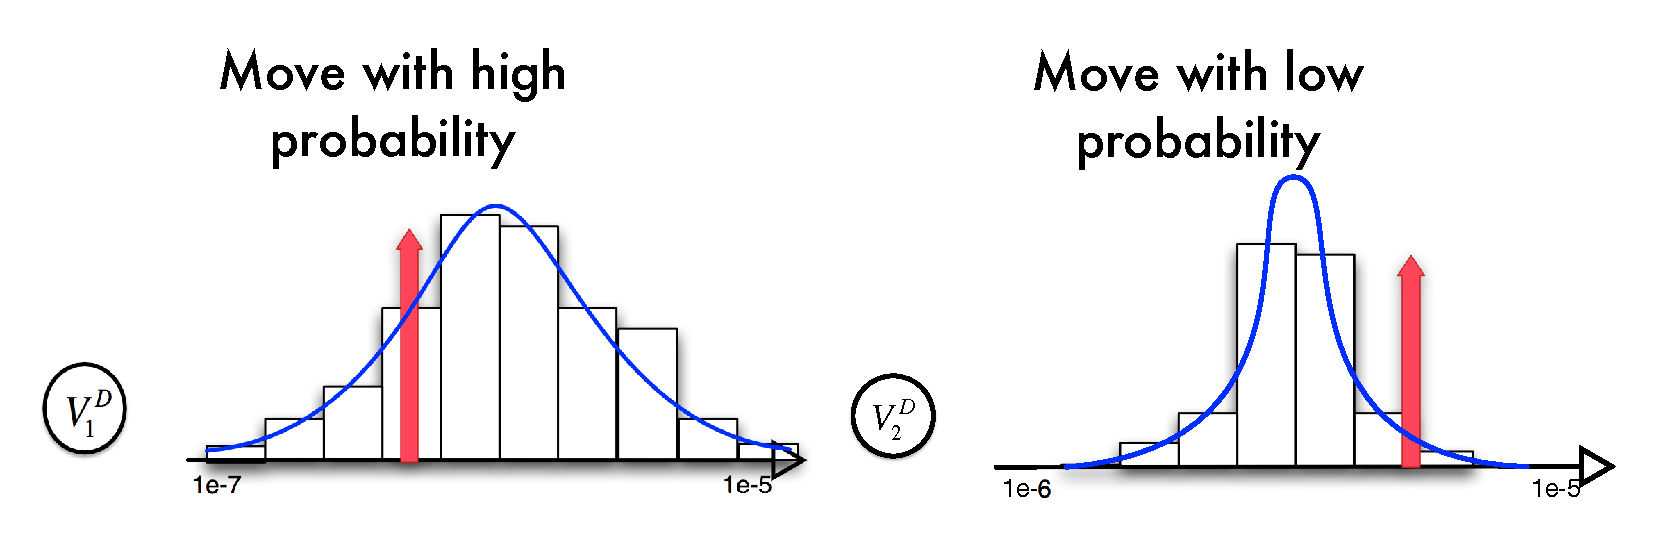
\includegraphics[width=\textwidth]{Fig/NorPDFSwap.eps}
    \caption{Swap behavior dominated by probabilistic in PDF of $V^D_m$} 
    \label{fig:NorPDFSwap}
  \end{figure}


  \newtheorem{PFTSDef}{Definition}
  %\newtheorem{Dominate}[func]{Definition}
  \begin{defi}\label{def:Dominate}
    x $\prec$ y (called x dominates y) iff $E_i(x)$ $\leq$ $E_i(y)$, for i=1,\dots ,K and $E_j(x)$ $\leq$ $E_j(y)$ for least one objective function $E_j$.
  \end{defi}

  \begin{defi}\label{def:objective}
    The composite objective function is defined, $E=\displaystyle\sum_{n=1}^{K} ln(w_if_i(x))$, where $f_1$, $\dots$ ,$f_K$ are K objectives to be optimized and $w_i$ is normalized weighting value corresponding to each objective result, for i=1, $\dots$ ,k.
  \end{defi}



  \section{Experimental Results}\label{sec:PAGEExp}

    To evaluate our methodology, two analog designs are practiced as our experimental targets. One is radio-frequency distributed amplifier(RFDA) in~\cite{PerfMap_ISQED2011} and the other is a folded cascode operational amplifier. As illustrated in Table~\ref{table:stat}, there are five performance targets to achieve for RFDA. These are voltage gain ($A_v$), DC power consumption ($P_{dc}$), output power ($P_{out}$), central frequency ($F_{cent}$) and bandwidth ($BW$), respectively. Similarly to Opamp, we measure 5 performance targets: voltage gain ($A_v$), DC power consumption ($P_{dc}$), output power ($P_{out}$), bandwidth ($BW$) and phase margin ($PM$), respectively. For technology migration purpose, both two circuits in the experiments also consider three technology processes: (1) umc65nm, (2) umc90nm and (3) tsmc90nm for different foundry model purposes. 
    \newsavebox{\tablebox}
    \begin{table}[ht]
      \begin{center}
      {\small
        \caption{Device statistics of RFDA and OpAmp}\label{table:stat}
        \begin{lrbox}{\tablebox}
          \centering{
            \begin{tabular}{|c|c|c|c|c|c|}
              \hline
              &  \multicolumn{5}{c|}{Device Number} \\
              \cline{2-6}
              circuits &  MOS &   Capacitor & Resistor  &  Inductor & Total   \\
              \hline
              RFDA     &  12   &   30       &     0     &     30     &   72     \\
              \hline  
              Spec     &  $A_v(\frac{v}{v})$    & $P_{dc} (\mu W)$  & $P_{out}(mW)$  & $F_{cent}(GHz)$ & $BW(GHz)$   \\ 
              \cline{2-6}  
                       &  $ \geq5$ & $\leq 0.5$ & $\geq 2$& $\geq 5$ & $\geq 10$ \\
              \hline  
              Opamp   &  18   &    1       &     0     &      0     &   19     \\
              \hline  
              Spec     &  $A_v(\frac{v}{v})$    & $P_{dc} (\mu W)$  & $P_{out}(\mu W)$ & $BW(MHz)$   & Phase Margin  \\
              \cline{2-6}  
               &  $ \geq40$ & $\leq 100$ & $\geq 0.1 $& $\geq 60$ & $\geq 50$ \\
              \hline
            \end{tabular}
          }
          \end{lrbox}
        \scalebox{0.8}{\usebox{\tablebox}}
        }
      \end{center}
    \end{table}

    \definecolor{mygray}{gray}{.9}
    \begin{sidewaystable}
      \begin{center}
      \caption{The mapping results from circuit-level variables to performance metrics and the runtime from circuit-level to performance metrics for \cite{PerfMap_ISQED2011} and 3 genetic exploration styles.}    
      \label{table:PopulationResult}
      \begin{lrbox}{\tablebox}
        \centering{
        \begin{small}
        \begin{tabular}{|l|l|c|c|c|c|c|c|c|}
            \hline
            \rowcolor{mygray}
            RFDA        & Algorithm &Runtime(s) & Rumtime Improv.&    $A_v(\frac{v}{v})$    & $P_{dc} (\mu W)$  & $P_{out}(mW)$  & $F_{cent}(GHz)$           & $BW(GHz)$   \\ 
            \hline
            \cline{2-9}
                    & {\bf ITE}\cite{PerfMap_ISQED2011} &  38880 & - & 1.5- 8 & $\leq 0.85$ & $\leq 21.7$ &  $2.6802 \sim 27.299$     & $ 2.3485 \sim 51.587$ \\
            \cline{2-9}
                    & $\text G\text A_{64}$  & 4122  & 9.43x& 4 \~ 5.2143 & 0.368 - 0.997 & 20.9 - 21.2 &   11.0 - 13.56   & 18.92 - 24.10 \\
            \cline{2-9}
             umc65nm    & $\text P\text G\text A_{64}$  & 3416 & 11.38x&  4 - 5.2143 & 0.354 - 0.990  &  20.9 - 21.2 & 11.04 - 13.56& 19.07 - 24.10 \\
             \cline{2-9}
                    & $\text P\text G\text A_{256}$  & 8053 & 4.82x  & 4 - 5.2298 & 0.002 - 1.019 & 20.9 - 27.8 &  11.12 - 13.52   & 19.23 - 23.94 \\
            \hline
            \rowcolor{mygray}
            Opamp        & Algorithm &Runtime(s) & Runtime Improv. &   $A_v(\frac{v}{v})$    & $P_{dc} (\mu W)$  & $P_{out}(mW)$  & $PM$  & $BW(MHz)$   \\ 
            \hline
            \cline{2-9}
                    & {\bf ITE}\cite{PerfMap_ISQED2011} & 19432  & -  & 20 - 32.26 & $\leq 100$ & $\leq 0.65$  &  30\textdegree $\sim$  60\textdegree & $0.08 \sim 1.47$ \\
            \cline{2-9}
                    & $\text G\text A_{64}$ & 5958  & 3.26x  & 10 - 65.71 & 14 $\sim$ 100 & 0.1 $\sim$ 0.87 &   30\textdegree $\sim$ 72.85\textdegree   & $0.08 \sim 1.5$ \\
            \cline{2-9}
             umc65nm    & $\text P\text G\text A_{64}$  &1855 & 10.48x &  10 $\sim$ 91 & 28 $\sim$ 100  &  0.1 $\sim$ 1 & 30\textdegree $\sim$ 66\textdegree   & $0.1 \sim 1.5$  \\
             \cline{2-9}
                    & $\text P\text G\text A_{256}$  & 7992 & 2.43x  & 10 $\sim$ 91 & 14 $\sim$ 100 & 0.1 $\sim$ 1 &  30\textdegree $\sim$ 81\textdegree  & $0.1 \sim 1.5$ \\
            \hline
            \cline{2-9}
                    & {\bf ITE}\cite{PerfMap_ISQED2011} &  15285 & - & $20 \sim 46.77$ & $\leq 100$ &$\leq 0.65$  & 30\textdegree $\sim$ 60\textdegree &$0.08 \sim 1.47$  \\
            \cline{2-9}
                    & $\text G\text A_{64}$   & 4858  & 3.15x& 10 $\sim$ 145 & $14 \sim 100$ & 0.23 $\sim$ 1 &   38.57\textdegree $\sim$ 72.85\textdegree   &0.1 $\sim$ 1 \\
            \cline{2-9}
             umc90nm    & $\text P\text G\text A_{64}$ & 1813 & 8.43x &  10 $\sim$ 118 & 14 $\sim$ 85  &  0.1 $\sim$ 0.75 & 30\textdegree $\sim$ 81\textdegree & 0.1 $\sim$ 1.5  \\
             \cline{2-9}
                    & $\text P\text G\text A_{256}$  & 4037 & 3.79x & 10 - 400 & 1.28 - 30 & 0.25 - 0.89 &  30\textdegree $\sim$ 60\textdegree & 0.48 $\sim$ 1.5 \\
            \hline
            \cline{2-9}
                    & {\bf ITE}\cite{PerfMap_ISQED2011} & 19488 & -   & 20 $\sim$ 34.15 & $\leq 0.1$ & $\leq 0.91$  & 30\textdegree $\sim$ 60\textdegree  & 0.08 $\sim$ 1.47 \\
            \cline{2-9}
                    & $\text G\text A_{64}$  & 5918  & 3.29x &10 - 74.29 & 0.05 - 29.7 & 0.12 - 1.03 &  30\textdegree $\sim$ 60\textdegree   & 0.48 $\sim$ 1.5 \\
            \cline{2-9}
             tsmc90nm    & $\text P\text G\text A_{64}$ & 2805 & 6.94x &  10 - 74.29 & 0.14 - 28.68  &  0.18 - 1.03 & 30\textdegree $\sim$ 60\textdegree& 0.48 $\sim$ 1.5 \\
             \cline{2-9}
                    & $\text P\text G\text A_{256}$  & 7108 & 2.74x  & 10 - 74.29 & 0.13 - 29.69 & 0.17 - 0.96 &  30\textdegree $\sim$ 60\textdegree & 0.48 $\sim$ 1.5 \\
            \hline

        \end{tabular}
        \end{small}
        }
        \end{lrbox}
        \scalebox{0.8}{\usebox{\tablebox}}
      \end{center}
    \end{sidewaystable} 


    Table~\ref{table:stat} shows the statistics of the two circuits including the components of each and the typical performance specifications. To examine the outcomes of proposed synthesis methodology, our experiments first analyze the performance exploration behavior with different evolution style in Section~\ref{sec:ExPerf}. Later, Section~\ref{sec:ExPSUniFT}, \ref{sec:ExPSProFT} and \ref{sec:ExPSGEFT} validate the efficiency for parallel evolution on genetic algorithm (PGA) and probabilistic stochastic fine-tuning. Our methodology is implemented in the environment of GCC version 4.3.4, Matlab Runtime Compiler 4.15, and the cvx optimization package. Also, to accelerate the framework, this algorithm also employee openMP and Matlab distributed computing toolbox for parallel computing purpose by rewriting the Matlab cvx package and the design equations of RFDA and Opamp are compiled as libraries into our C++ based parallel genetic algorithm. All of the implementation is accomplished under one Intel Xeon E5620 2.4GHz machine with 72GB memory.
      
    

    \subsection{Performance Exploration Stage}\label{sec:ExPerf}

      To validate the efficiency of parallel genetic exploration for circuit performance mentioned in Section~\ref{sec:pga}. We compare it to the following methods: 
      \begin{enumerate}
          \item {\bf ITE}, a iterative searching approach which carefully traverse every performance metrics combination. 
          \item {$\bf GA_{64}$}, a pure genetic algorithm based performance exploration with total population size $N_P=64$. $GA_{64}$ evolve the population each performance target independently. 
          \item {$\bf PGA_{64}$}, a multi-objective parallel genetic algorithm based performance exploration with total population size $N_P=64$ and 5 sub-populations
          \item {$\bf PGA_{256}$}, a multi-objective parallel genetic algorithm based performance exploration with total population size of $N_P=256$ and 5 sub-populations.
      \end{enumerate}

      As listed in Table~\ref{table:PopulationResult}, we also consider the previous performance exploration approach in \cite{PerfMap_ISQED2011}, which exhaustively search the range of each performance metrics. Both for RFDA and OpAmp case, there are five performance requirement should be examined. We traverse each performance metric with five value from low to high. Thus, there are $5^5$ combination of performance configurations. {\bf} ITE will evaluate each performance metric to figure out the Pareto front curve. Table~\ref{table:PopulationResult} lists the results of the runtime and performance boundary we have traversed.

      Obviously, {\bf ITE} costs the most runtime for evaluating $5^5$ points of performance configuration. Averagely, {\bf ITE} takes more than 10,000sec for performance exploration. Meanwhile, genetic exploration for performance space is much faster. {$\bf GA_{64}$} explores 9.43x, 3.26x, 3.15x and 3.29x times faster over {\bf ITE} under RFDA-umc65nm, Opamp-umc65nm, Opamp-umc90nm and Opamp-tsmc90nm circuits respectively. {$\bf PGA_{64}$} even performs 11.38x, 10.48x, 8.43x and 6.94x times faster than {\bf ITE} approach under RFDA-umc65nm, Opamp-umc65nm, Opamp-umc90nm and Opamp-tsmc90nm circuits respectively. In {\bf $PGA_{256}$} case, which explores twice volume of population, it increase the runtime a bit, but all of them are still faster than {\bf ITE} over 4.82x, 2.43x, 3.79x and 2.74x times under RFDA-umc65nm, Opamp-umc65nm, Opamp-umc90nm and Opamp-tsmc90nm circuits, respectively. 

      Since {\bf ITE} should traverse the given performance space carefully to check the feasibility, the searching procedure takes longer runtime. Moreover, the range of performance space is non-deterministic. The Pareto-Front of the circuit behavior is selected manually. Unlike {\bf ITE}, all of the genetic explorations converge the performance space much closer. Since genetic algorithm based approach select the population with higher fitness, the solution space tends to be more specific. We will verify the correctness with simulation in Section~\ref{sec:ExPSUniFT}, \ref{sec:ExPSProFT} and \ref{sec:ExPSGEFT}.
      
      Among three genetic exploration, {$\bf GA_{64}$}, {$\bf PGA_{64}$} and {$\bf PGA_{256}$}, there are a few differentiation in explored performance spaces. Even though {$\bf PGA_{64}$} spends less runtime than {$\bf PGA_{256}$}, it achieves almost the same exploration result with {$\bf PGA_{256}$}'s. We can see the efficiency that PGA converges the performance space well with smaller population scope. 

  %\begin{comment}
    %\begin{table}
    %  \begin{center}
      
    %  \caption{Best performance of population results for RFDA and Opamp circuit with umc65nm, umc90nm and tsmc90nm technologies on $\text G\text A_{64}$, $\text P\text G\text A_{64}$ and $\text P\text G\text A_{256}$ based performance exploration.}    \label{table:BestResult}
    %  \begin{lrbox}{\tablebox}
    %  \centering{
    %  \begin{small}
    %  \begin{tabular}{|l|l|c|c|c|c|c|}
    %      \hline
    %      \rowcolor{mygray}
    %      RFDA        & Algorithm&    $A_v(\frac{v}{v})$    & %$P_{dc} (\mu W)$  & $P_{out}(mW)$  & $F_{cent}(GHz)$           & $BW(GHz)$   \\ 
    %     \hline
    %      \cline{2-7}
    %              & $\text G\text A_{64}$     & 5.2143 & 0.7218 & 21.2 &   11.2   & 19.2 \\
    %      \cline{2-7}
    %       umc 65nm    & $\text P\text G\text A_{64} $   &  5.2143 & 0.7465  &  21.2 & 11.3& 20.0 \\
    %       \cline{2-7}
    %              & $\text P\text G\text A_{256}$     & 5.2285 & 0.002 & 26.9 &  13.5   & 23.0 \\
    %      \hline
    %      \rowcolor{mygray}
    %      Opamp        & Algorithm&    $A_v(\frac{v}{v})$    & $P_{dc} (\mu W)$  & $P_{out}(\mu W)$  & $F_{cent}$           & $BW$   \\ 
    %      \hline
    %      \cline{2-7}
    %              & $\text G\text A_{64}$     & 65.71 & 33 & 0.90 &   4183   & 5019 \\
    %      \cline{2-7}
    %       umc 65nm    & $\text P\text G\text A_{64}$  &65.71 &33  &  0.90 & 4180   & 5020 \\
    %       \cline{2-7}
    %              & $\text P\text G\text A_{256}$     & 65.71 & 33 & 0.90 &  4183 & 5109 \\
    %      \hline
    %      \cline{2-7}
    %              & $\text G\text A_{64}$     & 65.71& 7.09 & 0.57 %&   3338   & 4006 \\
    %      \cline{2-7}
    %       umc 90nm    & $\text P\text G\text A_{64}$  &  65.71& 7.03  &  0.61 & 3455& 4146 \\
    %       \cline{2-7}
    %              & $\text P\text G\text A_{256}$     & 65.71 & 7.09 & 0.57 &  3338 & 4006 \\
    %      \hline
    %      \cline{2-7}
    %              & $\text G\text A_{64}$     & 35.71  & 7.6 & 0.587 &  3387   & 4064 \\
    %      \cline{2-7}
    %       tsmc 90nm    & $\text P\text G\text A_{64}$  &  48.57 & 12.18  &  0.54 & 3244& 3892 \\
    %       \cline{2-7}
    %              & $\text P\text G\text A_{256}$     & 35.71 & 8.81 & 0.68 & 3644 & 4373 \\
    %      \hline
    %  \end{tabular}
    %  \end{small}
    %  }
    %  \end{lrbox}
    %  \scalebox{0.8}{\usebox{\tablebox}}
  %\end{center}
  %\end{table}
  %\end{comment}


    \subsection{Fine-tuning Simulation Setup}\label{sec:ExPSFTSetting}  
      
      \begin{table}
        \begin{center}
        \caption{The performance exploration results for RFDA and Opamp circuit with umc65nm, umc90nm and tsmc90nm technologies on {\bf UniSA}, {\bf ITE+UniSA}, {$\bf GA_{64}$\bf+ProSA}, {$\bf PGA_{64}$\bf+UniSA}, {$\bf PGA_{64}$\bf+ProSA}, {$\bf PGA_{256}$\bf+UniSA}. and {$\bf PGA_{256}$\bf+ProSA} frameworks.}    \label{table:PerformanceResult}
        \begin{lrbox}{\tablebox}
        \centering{
        \begin{small}
        \begin{tabular}{|l|l|c|c|c|c|c|c|c|}
          \hline
          \rowcolor{mygray}
          RFDA        & Algorithm        & Runtime(s)& Runtime Improv.&    $A_v(\frac{v}{v})$    & $P_{dc} (\mu W)$  & $P_{out}(mW)$  & $F_{cent}(GHz)$           & $BW(GHz)$   \\ 
          \hline
          & {\bf ITE+UniSA}  & 38880 & 1& 6.4322    & 0.23  & 2.65  & 9.85  & 17.48 \\  
          \cline{2-9}
          & {$\bf GA_{64}$\bf+ProSA}  & 9756.02 & 3.98x  & 7.38 & 0.175 & 23.3 &   20.9   & 40.2 \\        
          \cline{2-9}
          umc 65nm    & {$\bf PGA_{64}$\bf+UniSA} & 6513 & 5.97x  & 1.1843 & 3.88 & 1.74 & 8.95 & 5.0 \\
           \cline{2-9}
          &  {$\bf PGA_{64}$\bf+ProSA} & 6300.15 &  6.17x &  8.505 &  0.183   &  18.8  & 22.5     & 40.4 \\
          \cline{2-9}
          & {$\bf PGA_{256}$\bf+UniSA}   & 12016 & 3.24x  & 2.2818 & 11.83 & 3.43 & 5.53 & 10.54\\
          \cline{2-9}
          & {$\bf PGA_{256}$\bf+ProSA}   & 11772 & 3.30x  & 6.1852 & 0.141 & 28.9 & 24 & 42.8 \\
          \hline
          \rowcolor{mygray}
          Opamp      & Algorithm     & Runtime(s)&  Runtime Improv.& $A_v(\frac{v}{v})$    & $P_{dc} (\mu W)$  & $P_{out}(\mu W)$ & $BW(MHz)$   & Phase Margin  \\ 
          \hline
          & {\bf UniSA} & 14699   &  1.32x  &  42.96&  93.75  &  0.27 & 97  &  76.8\textdegree\\
          \cline{2-9}
          & {\bf ITE+UniSA} & 19432   &  1  &  45.73&  102  &  0.21 & 144  &  45.7\textdegree\\
          \cline{2-9}
          &{$\bf GA_{64}$\bf+ProSA}&   8568 & 2.27x &  44.88& 93.76 & 0.428   &  102 & 67.84\textdegree  \\
          \cline{2-9}
          umc 65nm &{$\bf PGA_{64}$\bf+UniSA}   & 5123 & 3.79x  & 43.641 & 88.652 & 0.263 & 57 & 87.5\textdegree \\
          \cline{2-9} 
          &{$\bf PGA_{64}$\bf+ProSA}  &  4987   & 3.89x &  41.3& 99.4 &2.35 &  110 & 78\textdegree   \\
          \cline{2-9}
          & {$\bf PGA_{256}$\bf+UniSA}   & 12106 & 1.60x  & 44.075 & 88.779 & 0.3723 & 57.7 & 77.9\textdegree\\
          \cline{2-9}
          & {$\bf PGA_{256}$\bf+ProSA}   & 11174 & 1.74x  & 42.24 & 90 & 1.08 &62.5 & 82.58\textdegree \\
          \hline
          & {\bf UniSA} & 16023   &  0.95x  &  40.68&  90.96  &  2.64 & 56  &  65.56\textdegree\\
          \cline{2-9}
          &{\bf ITE+UniSA}  &  15285 &   1    & 33.16 & 95.6  &  1.72  & 78.58   &  65.872\textdegree  \\
          \cline{2-9}
          &{$\bf GA_{64}$\bf+ProSA} &  8797   &  1.73x  & 44.247&  96.36& 0.38  & 111   & 74.45\textdegree \\
          \cline{2-9}
          umc 90nm  &  {$\bf PGA_{64}$\bf+UniSA}  & 5012 & 3.05x  & 44.075 & 88.779 & 0.37 & 57.7 & 77.9\textdegree \\
          \cline{2-9}
          &{$\bf PGA_{64}$\bf+ProSA} &  4932 &  3.10x  & 44.68 &  93.3 & 1.2   & 87.4   &  74.5\textdegree \\
          \cline{2-9}
          & {$\bf PGA_{256}$\bf+UniSA}    & 7120 & 2.15x & 45.715 & 91.732  & 0.296 & 85.3 & 73.7\textdegree \\
          \cline{2-9}
          & {$\bf PGA_{256}$\bf+ProSA}   & 6818 & 2.24x  & 43.94 & 94.4 & 2.38 & 88.9 & 76\textdegree \\
          \hline
          \cline{2-9}
           & {\bf UniSA} & 17860   &  1.09x  &  41.88&  89.584  &  1.39 & 58  &  121.5\textdegree\\
          \cline{2-9}
           &{\bf ITE+UniSA}  &   19488    &   1    &  38.42& 111 & 1.2   & 284    &  50\textdegree   \\
          \cline{2-9}
           &{$\bf GA_{64}$\bf+ProSA}&   8703  &  2.24x  & 40.46 & 100.1 &  0.27 & 100   & 82\textdegree    \\
          \cline{2-9}
          tsmc 90nm &  {$\bf PGA_{64}$\bf+UniSA}   & 4902& 3.97x  & 39.282 & 91.1 & 0.43 & 64 & 86.07\textdegree \\
           \cline{2-9}
          & {$\bf PGA_{64}$\bf+ProSA}&   4651  &  4.19x &  39.28    &  93.3   &  1.16   &  70.4   &   85.5\textdegree    \\ 
          \cline{2-9}
          & {$\bf PGA_{256}$\bf+UniSA}   & 10638 & 1.83x & 28.858 & 87.21 & 2.90 & 28.02 &  91.17\textdegree\\
          \cline{2-9}
          & {$\bf PGA_{256}$\bf+ProSA}  & 10507 & 1.85x  & 40.72 & 89.4 & 1.13 & 71.2 & 86.52\textdegree \\
          \hline
        \end{tabular}
        \end{small}
        }
        \end{lrbox}
        \scalebox{0.8}{\usebox{\tablebox}}
        \end{center}
      \end{table}

      As we have already obtained performance spaces with above approaches, the re-targeting fine tuning simulation validates the performance results. In this paper, we provide 1) uniform swapping simulation and 2) probabilistic swapping simulation. 
      Since genetic exploration offers a set of design variable distributions.
      These distributions is suitable for probabilistic simulation to find optimized solution efficient. Here we list the combination of performance exploration approaches and simulation techniques as follows:

      \begin{enumerate}
        \item {\bf UniSA}, a multi-objective simulated annealing method referring to Suman et al. in \cite{MOSA}. We select random values for each design variables as an initial solution, then UniSA will search the final solution.
        \item {\{$\bf ITE,GA_{64},PGA_{64},PGA_{256}$\}\bf+UniSA}, four different performance explorations are accompanied with {\bf UniSA} for fine tuning. {\bf UniSA} starts the perturbation with an initial solution which is provided by performance exploration. 
        \item {\{$\bf GA_{64},PGA_{64},PGA_{256}$\}\bf+ProSA}, three genetic performance explorations are accompanied with probabilistic SA simulation. {\bf ProSA} starts the perturbation with different distributions of design variables for probabilistic perturbation provided by genetic explorations. 
      \end{enumerate}


      To figure out the impact from simulation style, we compare the same simulation type with different performance exploration results. Also, different simulations toward the same performance exploration style are considered. Like above experiences in Table~\ref{table:PopulationResult}, RFDA-umc65nm, Opamp-umc65nm, Opamp-umc90nm and Opamp-tsmc90nm are evaluated with these simulation styles. Table~\ref{table:PerformanceResult} illustrates the comparison of overall runtime, runtime improvement and performance metrics for different simulation styles with different target circuits.
    
    \subsection{Different Performance Exploration with Uniform Fine Tuning Comparison}\label{sec:ExPSUniFT}

      Among {\bf UniSA}, {\bf ITE+UniSA}, {$\bf PGA_{64}$\bf+UniSA} and {$\bf PGA_{256}$\bf+UniSA}, we focus on the effect from different performance exploration approaches with the same uniform SA simulation. Comparing between {\bf UniSA} and {\bf ITE+UniSA}, {\bf ITE+UniSA} benefits not much on runtime and performance metrics than {\bf UniSA}. While we manipulate {\bf UniSA} and {\bf ITE+UniSA} in almost the same runtime, it is not convincible that the hierarchical synthesis contributes to explore the optimal solution of analog circuit design. As illustrated in Table~\ref{table:PerformanceResult}, {\bf ITE+UniSA} obtains the worst PM and $P_{dc}$ with Opamp-umc65nm, the worst $A_v$ with Opamp-umc90nm and the worst PM with Opamp-tsmc90nm circuit. Obviously, the runtime is improved by parallel hierarchical synthesis strategies in {$\bf PGA_{64}$\bf+UniSA} and {$\bf PGA_{256}$\bf+UniSA}. Even though the parallel hierarchical synthesis methodologies need two stages to obtain optimal solutions, a full-circuit simulation takes more time to converge the solution space for good quality. 

      Table~\ref{table:PerformanceResult} illustrates more apparent differentiation among iterative exploration and parallel genetic exploration with {\bf UniSA}. Between {\bf ITE+UniSA} and {$\bf PGA_{64}$\bf+UniSA}, the runtime has been developed with 3.79x in Opamp-umc65nm, 3.05x in Opamp-umc90nm and 3.97x in Opamp-tsmc90nm. {$\bf PGA_{256}$\bf+UniSA} spends more time since the population is duplex. Between {\bf ITE+UniSA} and {$\bf PGA_{256}$\bf+UniSA}, the runtime has been developed with 1.60x in Opamp-umc65nm, 2.15x in Opamp-umc90nm and 1.83x in Opamp-tsmc90nm. Additionally, approaches with parallel genetic algorithm accomplish balanced performance metrics in Opamp circuits. But they obtain worse results in RFDA-umc65nm circuit. To sum up, the runtime of overall framework has been improved by performance exploration exploration stage, which reduce the convergent cost of circuit simulation and we can observe the efficiency of parallel genetic algorithm strategy. However, the overall performance does not reach the Pareto-front as expectation after UniSA simulation. We can observe that the uniform circuit simulation doesn't effectively propagate the good initial solution to the end. 

    \subsection{Different Parallel Genetic Exploration with Probabilistic Fine Tuning Comparison}\label{sec:ExPSProFT}

      Among {$\bf GA_{64}$\bf+ProSA}, {$\bf PGA_{64}$\bf+ProSA} and {$\bf PGA_{256}$\bf+ProSA}, we compare the runtime and performance results from different genetic exploration approaches with probabilistic SA simulation. According to each circuit in Table~\ref{table:PerformanceResult}, {$\bf PGA_{64}$\bf+ProSA} has better runtime results than {$\bf GA_{64}$\bf+ProSA} with the same size of population in all case of circuits. In RFDA-umc65nm, {$\bf PGA_{64}$\bf+ProSA} obtains 1.55x faster than {$\bf GA_{64}$\bf+ProSA} and 1.87x faster than {$\bf PGA_{256}$\bf+ProSA}. In Opamp circuit, {$\bf PGA_{64}$\bf+ProSA} earns the best runtime then the others. {$\bf GA_{64}$\bf+ProSA} takes the second place in umc65nm and tsmc90nm. We can tell that our approach achieves excellent runtime on {$\bf PGA_{64}$\bf+ProSA}.

      Beyond the runtime comparison, we also examine the performance metrics in each circuits on different genetic exploration styles with {\bf ProSA}. In RFDA-umc65nm, {$\bf PGA_{64}$\bf+ProSA} receives greatest $A_v$ with 8.505($\frac{v}{v}$), but its $P_{dc}$ is larger than {$\bf GA_{64}$\bf+ProSA} and {$\bf PGA_{64}$\bf+ProSA}. Other than $A_v$, {$\bf PGA_{256}$\bf+ProSA} obtains better $P_{dc}$, $P_{out}$, $F_{cent}$ and $BW$ than other genetic exploration styles with {\bf ProSA}. Obviously, all the genetic exploration styles with {\bf ProSA} have much better performance results than {\bf UniSA}. To sum up, {\bf ProSA} can discover good solution space for circuit RFDA-umc65nm efficiently. 

      In circuit Opamp circuits, three technologies achieve different results. On Opamp-umc65nm, {$\bf GA_{64}$\bf+ProSA} has better $A_v$ than the others, {$\bf PGA_{64}$} has better $P_{out}$ and $BW$. {$\bf PGA_{256}$} are superior to the others on $P_{dc}$ and $PM$. On Opamp-umc90nm, {$\bf GA_{64}$+ProSA} has better $BW$, {$\bf PGA_{64}$+ProSA} has better $A_v$ and $P_{dc}$, and {$\bf PGA_{256}$+ProSA} obtains great $P_{out}$ and $PM$. On Opamp-tsmc90nm, {$\bf GA_{64}$+ProSA} achieves better $BW$, {$\bf GA_{64}$+ProSA} obtains superior $P_{out}$, and {$\bf PGA_{256}$+ProSA} carries out good $A_v$, $P_{dc}$ and $PM$ than the others. As Table~\ref{table:PerformanceResult} illustrated, {$\bf PGA_{256}$\bf+ProSA} earns slightly better performance than $\bf PGA_{64}$ but it also costs twice runtime than $\bf PGA_{64}$. We can tell that the parallel genetic exploration has good efficiency on fewer population to gain the balanced performance metrics.

    \subsection{Different Fine Tuning with the Same Genetic Exploration Comparison}\label{sec:ExPSGEFT}

      Considering the same genetic exploration with different SA simulation techniques, such as{$\bf PGA_{64}$\bf+ProSA} and {$\bf PGA_{64}$\bf+UniSA}, the performance results are slightly different. Comparing to all the results generated by {\bf UniSA}, all the results with {\bf ProSA} achieve balanced performance metrics. {\bf ITE+UniSA} gets worse circuit stability with $PM=45.7$\textdegree, {$\bf GA_{64}$+UniSA} and {$\bf PGA_{64}$+UniSA} obtain worse $BW$ than the same genetic exploration style with {\bf ProSA}. The advantage of balanced performance can also be evaluated on different technologies node. On umc90nm, {\bf ITE+UniSA} obtains the worst $A_v$ performance results. Also, {$\bf PGA_{64}$+UniSA} and {$\bf PGA_{256}$+UniSA} get the worst $P_{out}$ performance results than the others. On tsmc90nm, {\bf ITE+UniSA} obtains the worst $PM$ with $50$\textdegree. In addition, {$\bf PGA_{256}$+UniSA} gets the worst $A_v$ and $BW$ with $28.858\frac{v}{v}$ and $28.02MHz$. Altogether, {\bf UniSA} achieves great performance in some performance targets but it backslide the other targets. We can tell that UniSA finds the local optimal solution.
    
      As seen in Table~\ref{table:PerformanceResult}, the results based on traditional simulation (as {\bf UniSA}) and iterative performance exploration (as {\bf ITE}) are not as good as ours. {\bf ITE} takes high runtime to search the performance space and {\bf UniSA} produces the performance results are unbalanced for all. Therefore, our improvements of parallel genetic exploration and probabilistic simulation are much more efficiency on performance searching and effective on converging to global optimal solution. In addition, the parallel genetic exploration performs high flexibility to search the performance domain in different population scale. Larger population size achieves better solutions but it also accompanies with more runtime. However, less population scale, such as {$\bf PGA_{64}$}, earns comparable solutions with much swifter runtime.
  
  \section{Summary}\label{sec:PAGESum}

    In this chapter, we address the performance space issue for advanced technologies in analog synthesis. We propose a hierarchical analog synthesis framework which integrates a parallel genetic algorithm based exploration and a probabilistic simulation. The parallel genetic exploration efficiently explores a potential performance space for optimal solution, and the probabilistic stochastic simulation proves adequate to search the global optimal with probabilities according to device variable distributions. This framework also minimizes runtime to converge the global optimal solution. As demonstration for our methodology, a RFDA circuit and an Op-Amp are practiced via 3 different technologies to show that our proposed performance exploration approach and probabilistic stochastic simulation commit comparable and balanced performance results with efficiency and accuracy for analog circuit synthesis.